% Settings for the default beamer theme
\documentclass[english, aspectratio=169]{beamer}
\usepackage[T1]{fontenc}
\usepackage[utf8]{inputenc}
\usepackage{tabularx}
\usepackage{babel}
\usepackage[ruled,vlined]{algorithm2e}
\SetAlgorithmName{Algoritmus}{algoritmus}{List of Algorithms}
\setcounter{secnumdepth}{3}
\setcounter{tocdepth}{3}

\makeatletter

\newcommand\makebeamertitle{\frame{\maketitle}}

% (ERT) argument for the TOC
\AtBeginDocument{%
  \let\origtableofcontents=\tableofcontents
  \def\tableofcontents{\@ifnextchar[{\origtableofcontents}{\gobbletableofcontents}}
  \def\gobbletableofcontents#1{\origtableofcontents}
}

% Theme settings
\usetheme{Frankfurt}
\usecolortheme{default}
\usefonttheme[onlymath]{serif}

% Template settings
\setbeamertemplate{navigation symbols}{}
\setbeamertemplate{blocks}[rounded][shadow=false]
\setbeamertemplate{title page}[default][colsep=-4bp, rounded=true, shadow=false]
\makeatother

\begin{document}

% Title page
\section{Bevezetés}
\title[]{Üzleti Intelligencia}
\subtitle{9. Előadás: Egyedek felismerése}
\author[Kuknyó Dániel]{Kuknyó Dániel\\Budapesti Gazdasági Egyetem}
\date{2023/24\\1.félév}
\makebeamertitle

% Table of contents slide
\begin{frame}
\tableofcontents{}
\end{frame}

% Table of contents of the current section
\begin{frame}
\tableofcontents[currentsection]
\end{frame}

\begin{frame}{Objektum lokalizáció}
\begin{columns}
\begin{column}{.5\textwidth}
A lokalizáció feladatában a modell nem csak egy címkét rendel hozzá a képhez valamilyen előre meghatározott címkehalmazból, hanem \textbf{megadja a keresett objektum kereteződobozának koordinátáit} is.\par\smallskip
Ezek a koordináták a $x,y,w,h$ vagyis a bal felső sarok $x,y$ koordinátái, a doboz szélessége és hosszúsága.\par\smallskip
A lokalizáló hálózatnak \textbf{két output rétege} (feje) van. Az egyik az objektum osztályba esésének valószínűségét adja meg, a másik pedig a dobozának koordinátáit.
\end{column}
\begin{column}{.5\textwidth}
\begin{center}
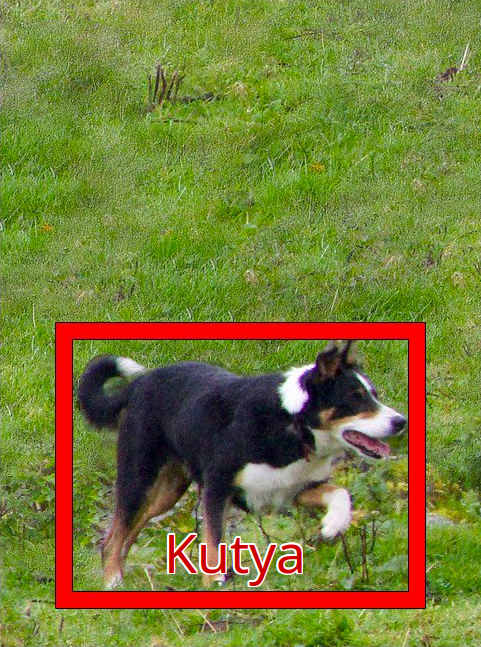
\includegraphics[height=6cm, width=7cm, keepaspectratio]{images/instance_11.png}
\end{center}
\end{column}
\end{columns}
\end{frame}

\begin{frame}{Objektum detekció}
\begin{columns}
\begin{column}{.5\textwidth}
Az objektum detekció a \textbf{lokalizáció általánosítása tetszőleges számú objektumra} egyetlen képen belül.\par\smallskip
Detekció esetén a neurális modell feladata megtalálni az \textbf{összes olyan objektumot, amely ismert} a címkehalmazban.\par\smallskip
Az objektum detektor outputja kereteződobozok és a hozzájuk tartozó válószínűségeloszlások halmaza, ezért \textbf{multioutput} osztályozási eljárásnak tekinthető.
\end{column}
\begin{column}{.5\textwidth}
\begin{center}
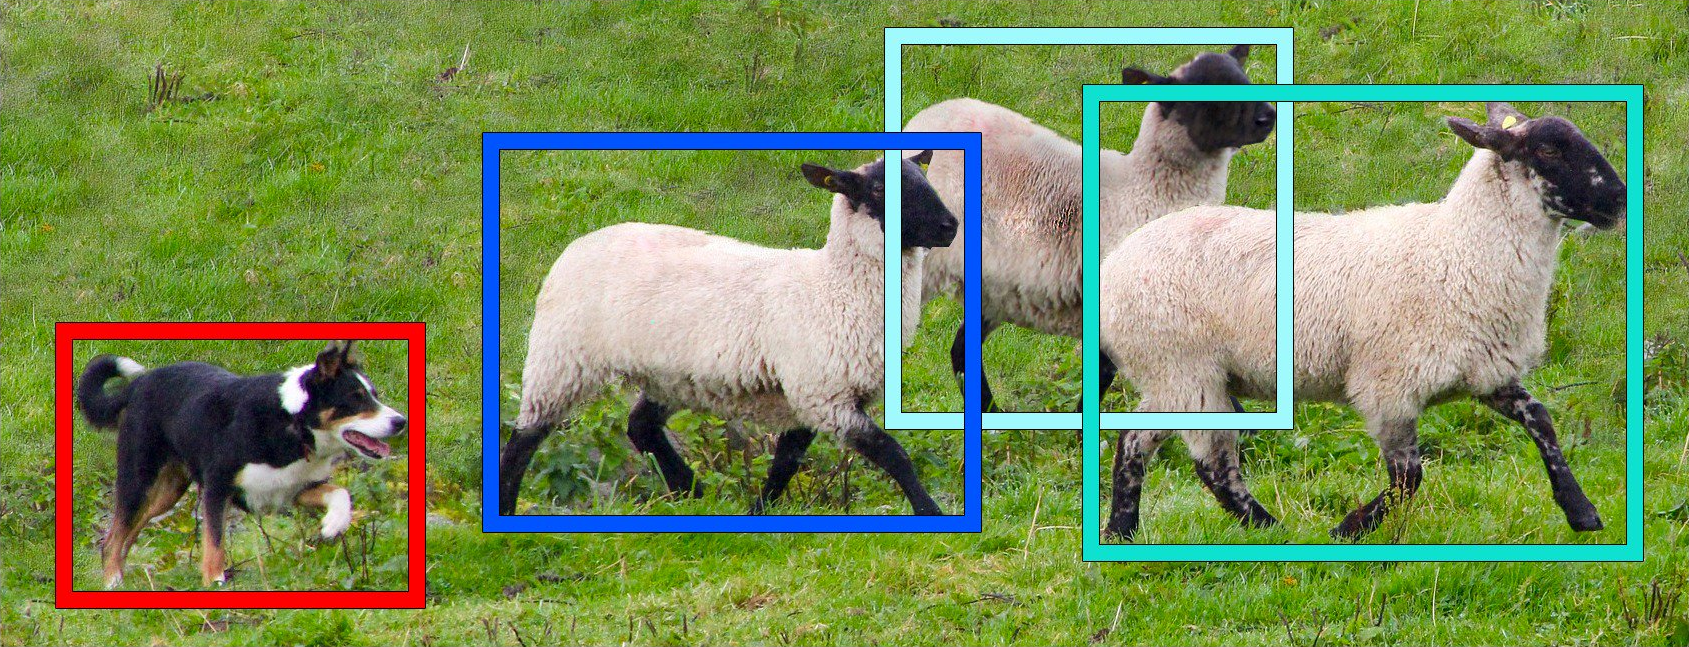
\includegraphics[height=5cm, width=7cm, keepaspectratio]{images/instance_3.png}
\end{center}
\end{column}
\end{columns}
\end{frame}

\begin{frame}{Szemantikus szegmentáció}
A szemantikus szegmentáció problémája nem csak megtalálni, hogy az egyes keresett objektum osztályoknak hol található a kereteződoboza a képen belül, hanem \textbf{pixel szinten osztályozást végezni a képen} belül a keresett objektumokra.\par\smallskip
\begin{columns}
\begin{column}{.5\textwidth}
\begin{block}{Szemantikus szegmentáció}
A szemantikus szegmentáció egy sűrű, pixelenkénti osztályozást ad outputként az input képre vonatkozóan \textbf{anélkül, hogy megkülönböztetné az objektumok egyedeit}. Az a pixel, amelyik nem becsülhető meg kellően magas valószínűséggel, osztályozatlanul marad.
\end{block}
\end{column}
\begin{column}{.5\textwidth}
\begin{center}
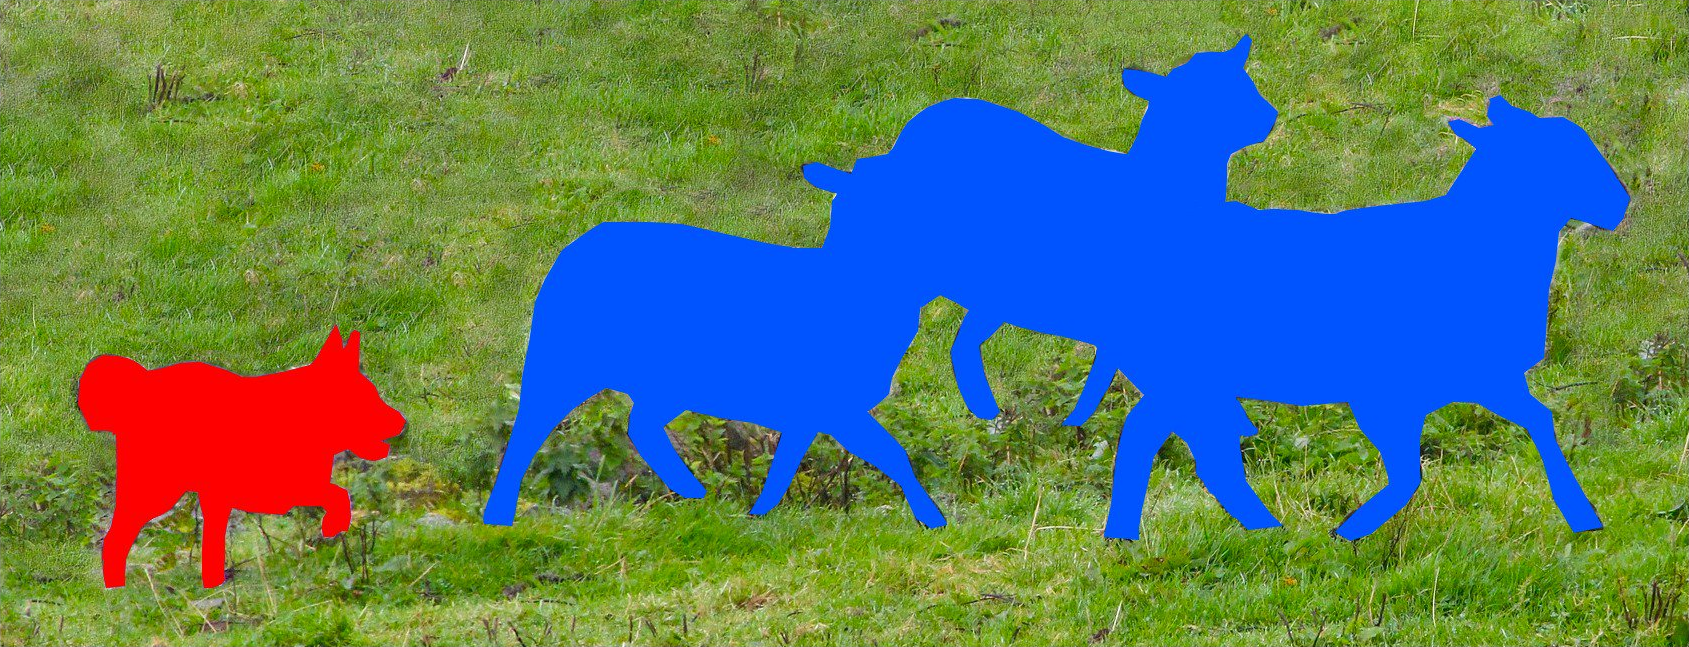
\includegraphics[height=7cm, width=7cm, keepaspectratio]{images/instance_4.png}
\end{center}
\end{column}
\end{columns}
\end{frame}

\begin{frame}{Pixelszintű osztályozás}
\begin{columns}
\begin{column}{.5\textwidth}
A szemantikus szegmentáció naív implementációja úgy működne, hogy egy \textbf{csúszóablak végigmegy a teljes képen}, és minden egyes pixelt végigáramoltat egy osztályozó neurális hálózaton.\par\smallskip
\textbf{Ez viszont lehetetlen}, mert egyetlen RGB színadat alapján nem lehet megmondani a képpont szemantikai jelentését.
\end{column}
\begin{column}{.5\textwidth}
\begin{center}
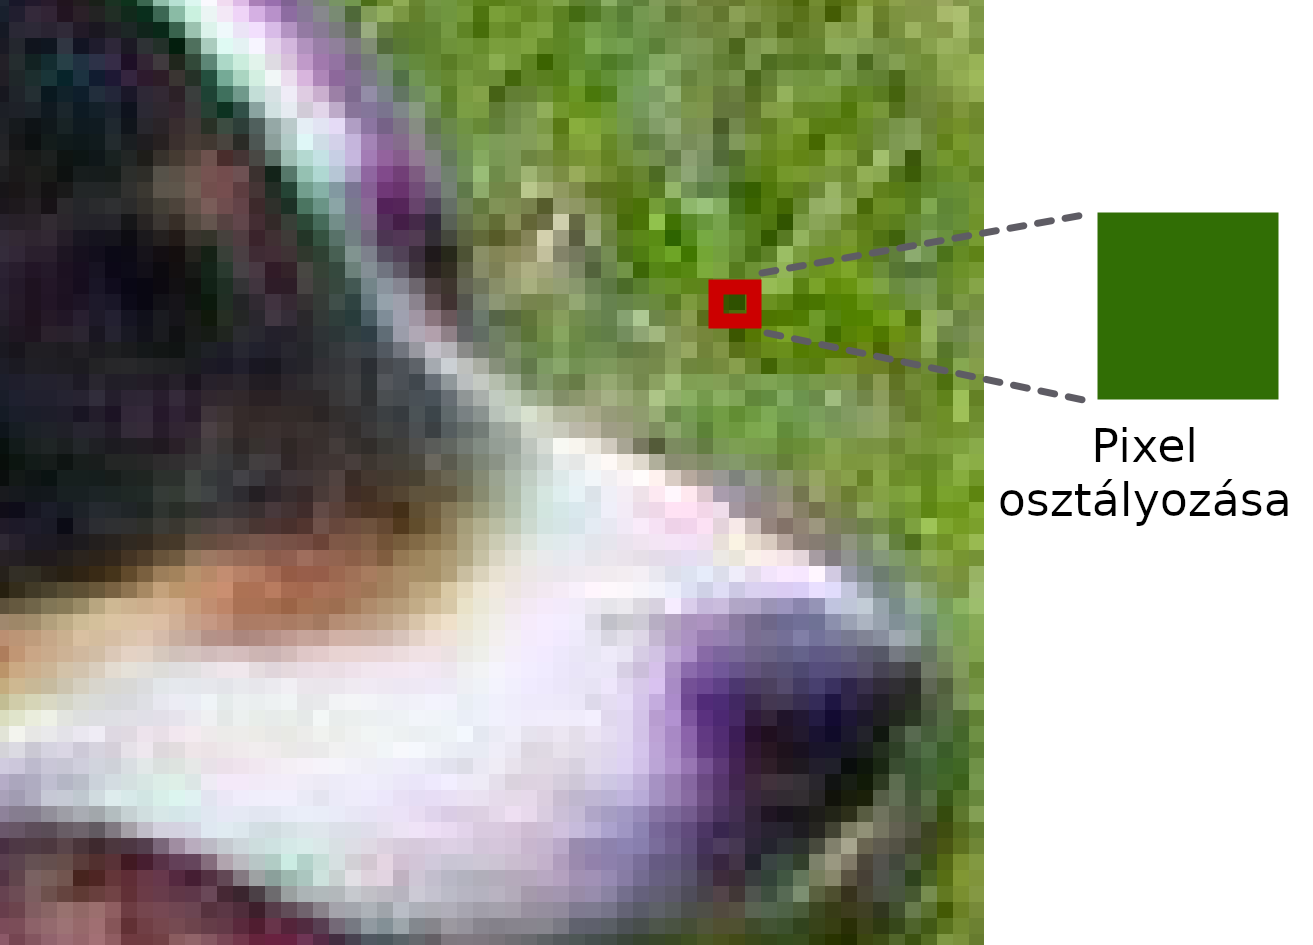
\includegraphics[height=7cm, width=7cm, keepaspectratio]{images/instance_7.png}
\end{center}
\end{column}
\end{columns}
\end{frame}

\begin{frame}{Ablakszintű osztályozás}
\begin{columns}
\begin{column}{.4\textwidth}
Egy másik naív megoldása a pixelszintű osztályozásnak, ha az algoritmus \textbf{végigmozgat egy ablakot a képen}, majd az ablakhoz tartozó régiót beosztályozza egy konvolúciós hálózat segítségével, majd az outputját hozzárendeli a középső pixelhez.\par\smallskip
A probléma ezzel a hozzáállással ismételten az, hogy \textbf{minden pixelre lefuttatni egy osztályozást rendkívül költséges}, a valóságban nem kivitelezhető.
\end{column}
\begin{column}{.6\textwidth}
\begin{center}
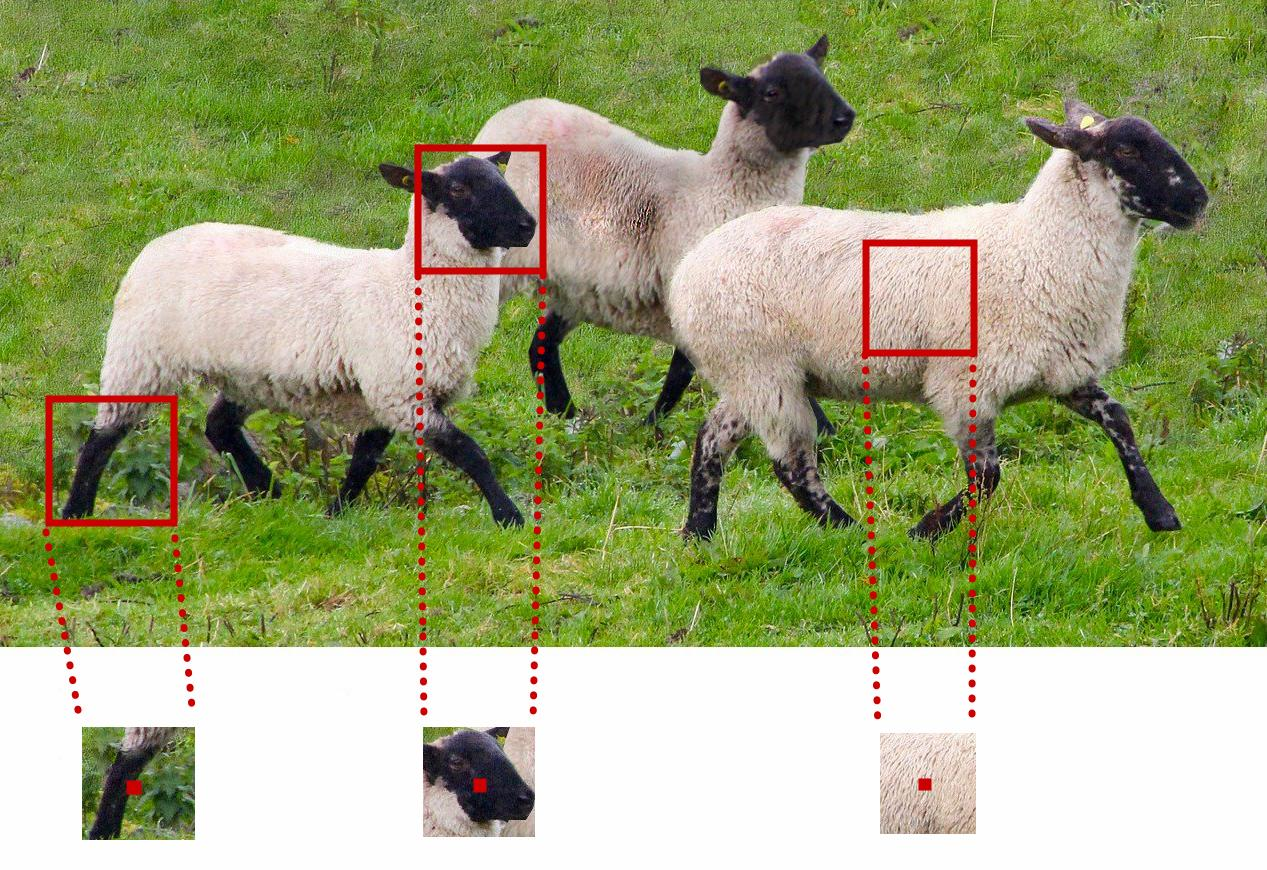
\includegraphics[height=10cm, width=8cm, keepaspectratio]{images/instance_8.png}
\end{center}
\end{column}
\end{columns}
\end{frame}

\begin{frame}{Szemantikus szegmentálás konvolúciós hálózattal}
Egy intuitív hozzáállás a szemantikus szegmentációhoz, hogy a modell \textbf{végigáramoltatja több konvolúciós rétegen az input képet}, majd az outputjából kiválasztja a legnagyobb valószínűségű osztályt minden egyes képpontra.\par\smallskip
Ebben az esetben az \textbf{output méretnek meg kell egyeznie az input mérettel}, ezért az összes konvolúciós szűrőnek azonos méretűnek kellene lennie! A teljes felbontású konvolúció ismételten egy nagyon költséges megoldás.  
\begin{center}
\vspace{.5cm}
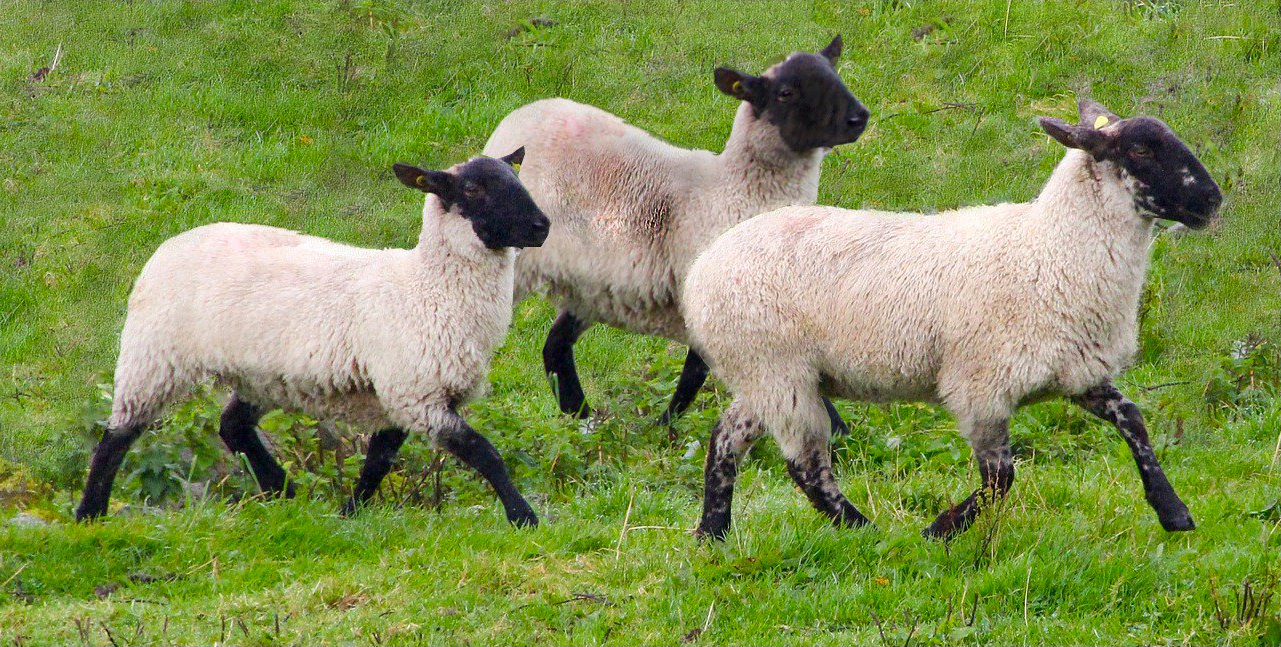
\includegraphics[width=3.25cm, keepaspectratio]{images/instance_9.png}
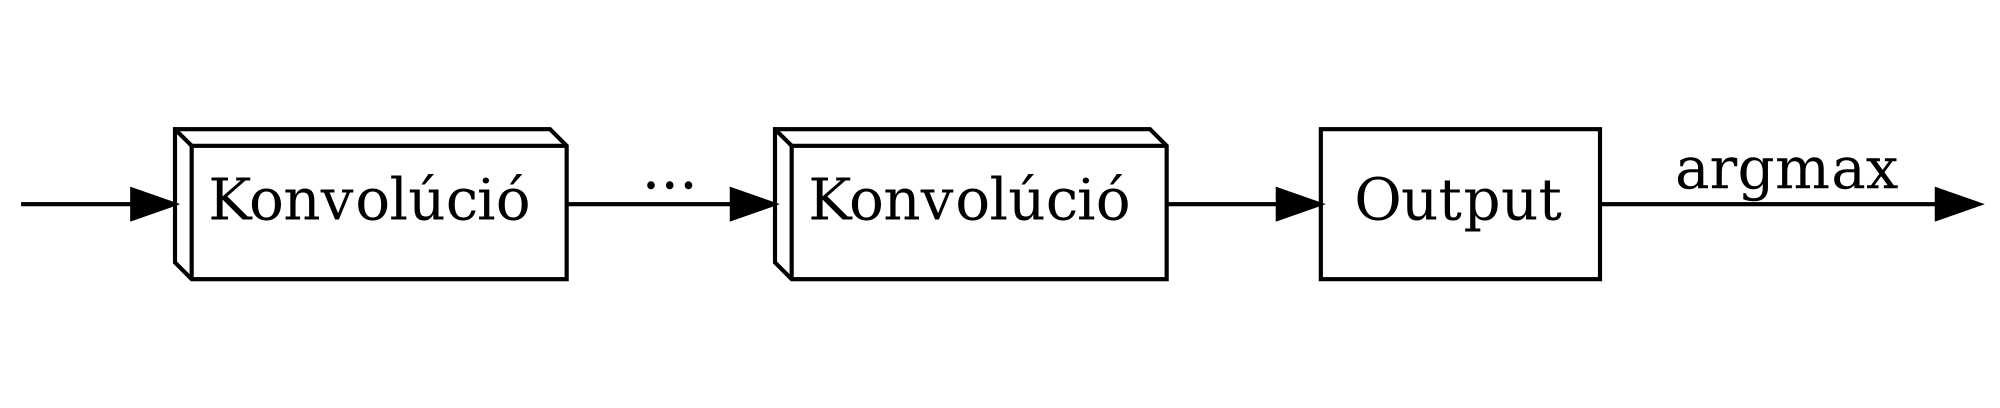
\includegraphics[width=7cm, keepaspectratio]{graphs/instance_1.png}
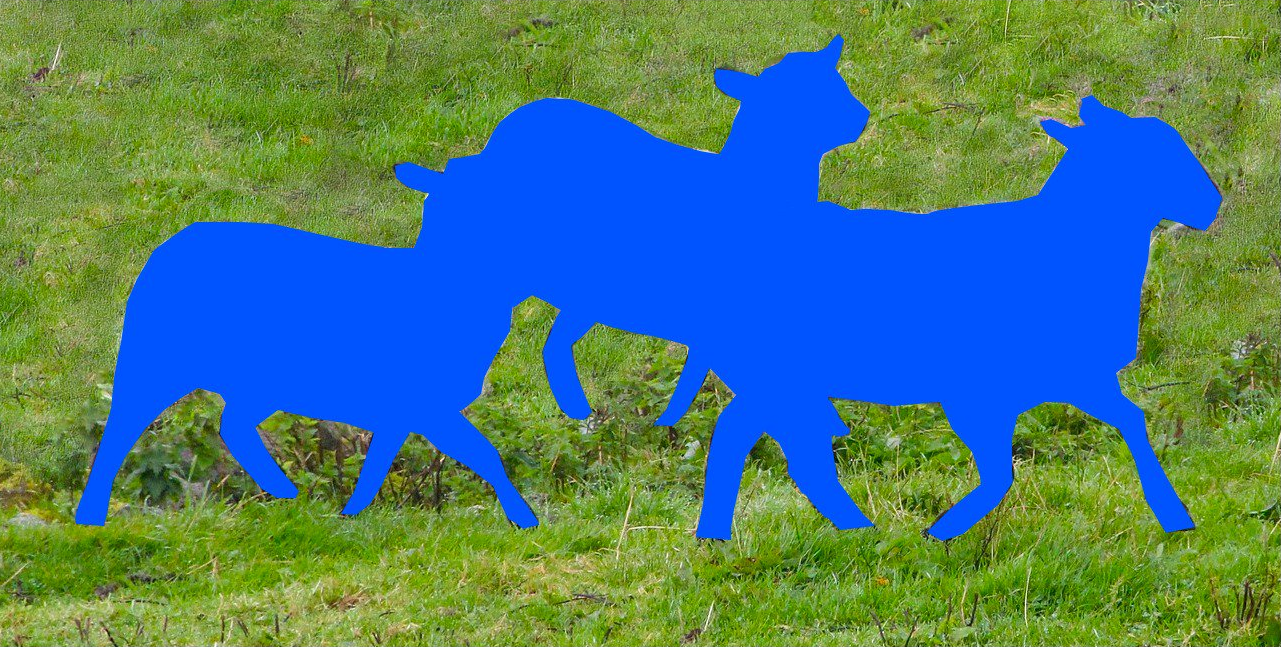
\includegraphics[width=3.25cm, keepaspectratio]{images/instance_10.png}
\end{center}
\end{frame}

\section{Szemantikus szegmentálás}

\begin{frame}
\tableofcontents[currentsection]
\end{frame}

\begin{frame}{Teljesen konvolúciós szemantikus szegmentálás}
A bevált hozzáállás a szemantikus szegmentáció problémájához, ha olyan konvolúciós hálózaton áramlik át az input adat, ami \textbf{először lefelé mintavételezi}, majd \textbf{felskálázza a képet}, ezzel eliminálva a többszörös teljes felbontású konvolúcióból adódó problémákat. 
\vspace{.5cm}
\begin{center}
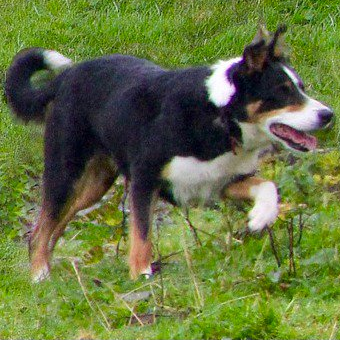
\includegraphics[height=3.15cm, keepaspectratio]{images/instance_13.png}
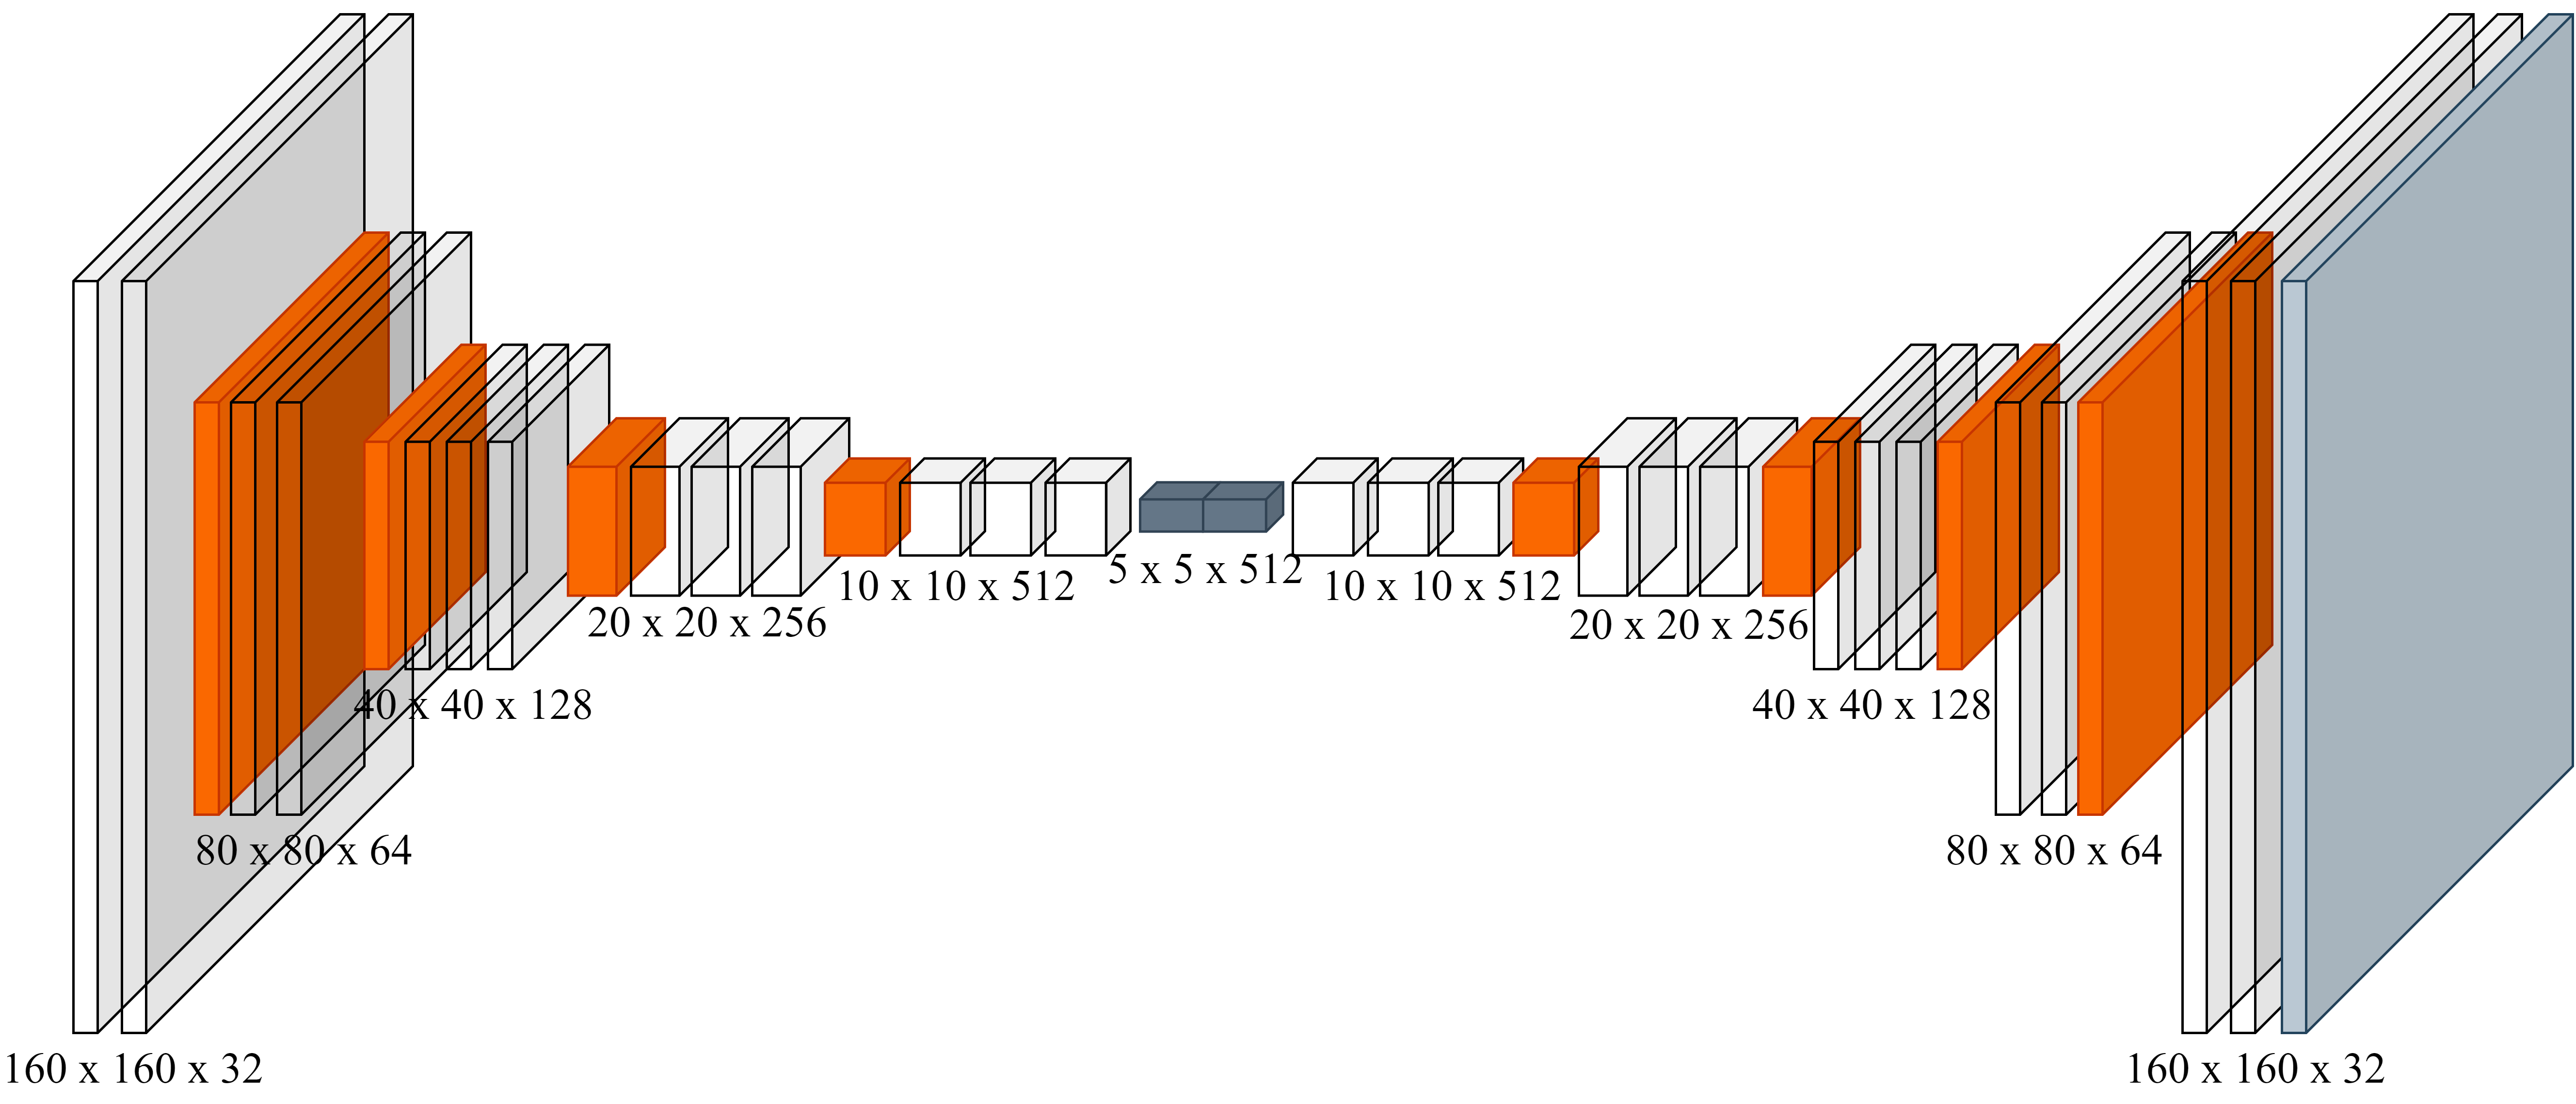
\includegraphics[height=3.15cm, keepaspectratio]{images/instance_12.png}
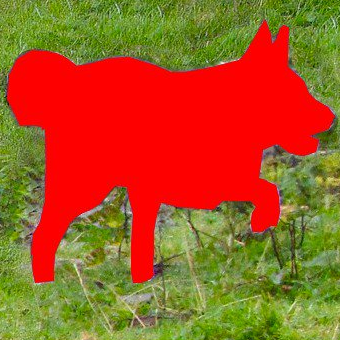
\includegraphics[height=3.15cm, keepaspectratio]{images/instance_14.png}
\end{center}
\end{frame}

\begin{frame}{Mintavételi eljárások}
\begin{columns}
\begin{column}{.5\textwidth}
\only<1>{\begin{block}{Lefelé mintavételezés}
A lefelé mintázó folyamatok az input adat térbeli dimenzióit hivatottak \textbf{csökkenteni} egy konvolúciós hálózatban a számítási teher csökkentése érdekében. Egy ilyen eljárás a \textbf{max. pooling}.\par\smallskip
Max. pooling során a réteg megőrzi a legnagyobb elemeket minden, a pooling neuronnal kapcsolatban álló bemenet közül.  
\end{block}}
\only<2>{\begin{block}{Felfelé mintavételezés}
A felfelé mintázó folyamatok az input adat térbeli dimenzióit hivatottak \textbf{növelni} egy konvolúciós hálózatban azért, hogy vissza lehessen nyerni felbontásban kódolt információt. Egy ilyen eljárás a \textbf{max. unpooling}.\par\smallskip
A max. unpooling során a lazított területek maximális elemei visszakerülnek azokra a pozíciókra, ahol eredetileg voltak. 
\end{block}}
\end{column}
\begin{column}{.5\textwidth}
\begin{center}
\includegraphics<1>[height=7cm, width=7cm, keepaspectratio]{images/instance_15.png}
\includegraphics<2>[height=7cm, width=7cm, keepaspectratio]{images/instance_16.png}
\end{center}
\end{column}
\end{columns}
\end{frame}

\begin{frame}{Felfelé mintavételezés}
Az output tartalmazza a szűrő másolatait a bemenet súlyozásával, \textbf{összegezve ott, ahol az átfedés van az outputban}. A felfelé mintavételezés művelete \textbf{értelmezhető tetszőleges dimenziószámra}. Ebben az esetben az $unpool(\cdot,\cdot)$ esetén az első paraméter az input, a második pedig a szűrő. A szűrő súlyai taníthatóak. 
\begin{center}
\[
unpool\left(\left[\begin{array}{c}
a\\
b
\end{array}\right],\left[\begin{array}{c}
x\\
y\\
z
\end{array}\right]\right)=\left[\begin{array}{c}
a\cdot x\\
a\cdot y\\
a\cdot z+b\cdot x\\
b\cdot y\\
b\cdot z
\end{array}\right]
\]
\end{center}
\end{frame}

\section{Egyed szegmentáció}

\begin{frame}
\tableofcontents[currentsection]
\end{frame}

\begin{frame}{Az egyed szegmentáció alapjai}
\begin{columns}
\begin{column}{.5\textwidth}
\begin{block}{Egyed szegmentáció}
Az egyed szegmentáció az egy képen található objektumokat \textbf{azonosítja és szegmentálja} olyan módon, hogy minden objektumhoz \textbf{külön maszkot rendel}.
\end{block}
\end{column}
\begin{column}{.5\textwidth}
\begin{center}
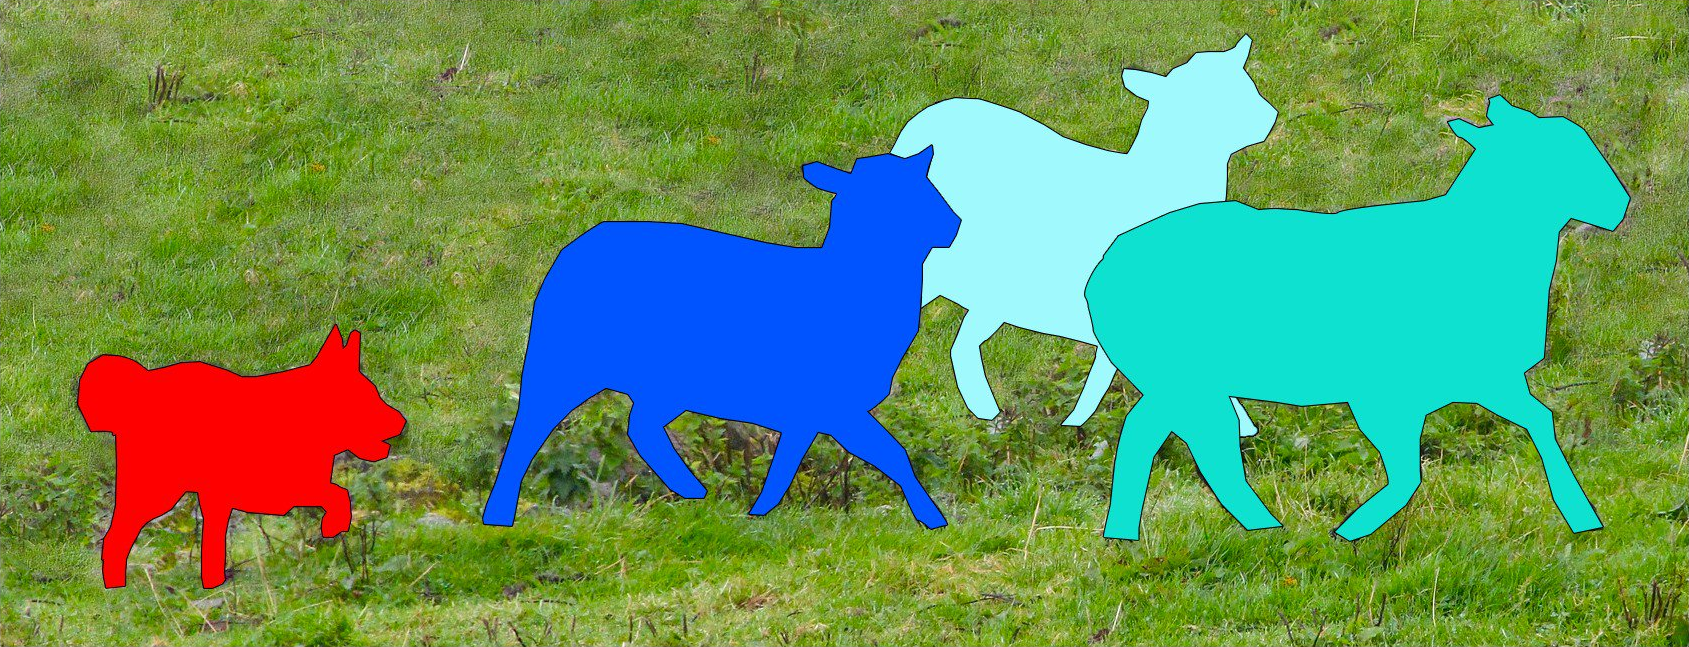
\includegraphics[height=7cm, width=7cm, keepaspectratio]{images/instance_5.png}
\end{center}
\end{column}
\end{columns}
\vspace{0.5cm}
Ez azt jelenti, hogy nem csak az objektumokat azonosítja (detekció), hanem a minden egyes objektumot \textbf{körülvevő pixel területeket is elkülöníti}. Az eredmény egy olyan maszk vagy maszkok halmaza, amely pontosan meghatározza a képen található egyedek \textbf{körvonalait és elhelyezkedését} a képen. 
\end{frame}

\begin{frame}{Objektum detektor és egyed szegmentáló architektúra}
\begin{columns}
\begin{column}{.5\textwidth}
\begin{itemize}
	\only<1->{\item \textbf{RPN osztályozás}: A kereteződoboz objektum / nem objektum?}
	\only<1->{\item \textbf{RPN regresszió}: A javasolt doboz és a kereteződoboz közötti transzformáció megbecslése.}
	\only<1->{\item \textbf{Objektum osztályozás}: A javaslatok osztályának megbecslése.}
	\only<1->{\item \textbf{Objektum regresszió}: A javasolt doboz és objektum doboz közötti transzformáció megbecslése.}
	\only<2>{\item \textbf{Maszk predikció}: Minden területi javaslatra egy $28 \cdot 28$ bináris maszkot becsül meg.}
\end{itemize}
\end{column}
\begin{column}{.5\textwidth}
\begin{center}
\only<1>{Objektum detektor hálózat (Faster R-CNN)\par\smallskip
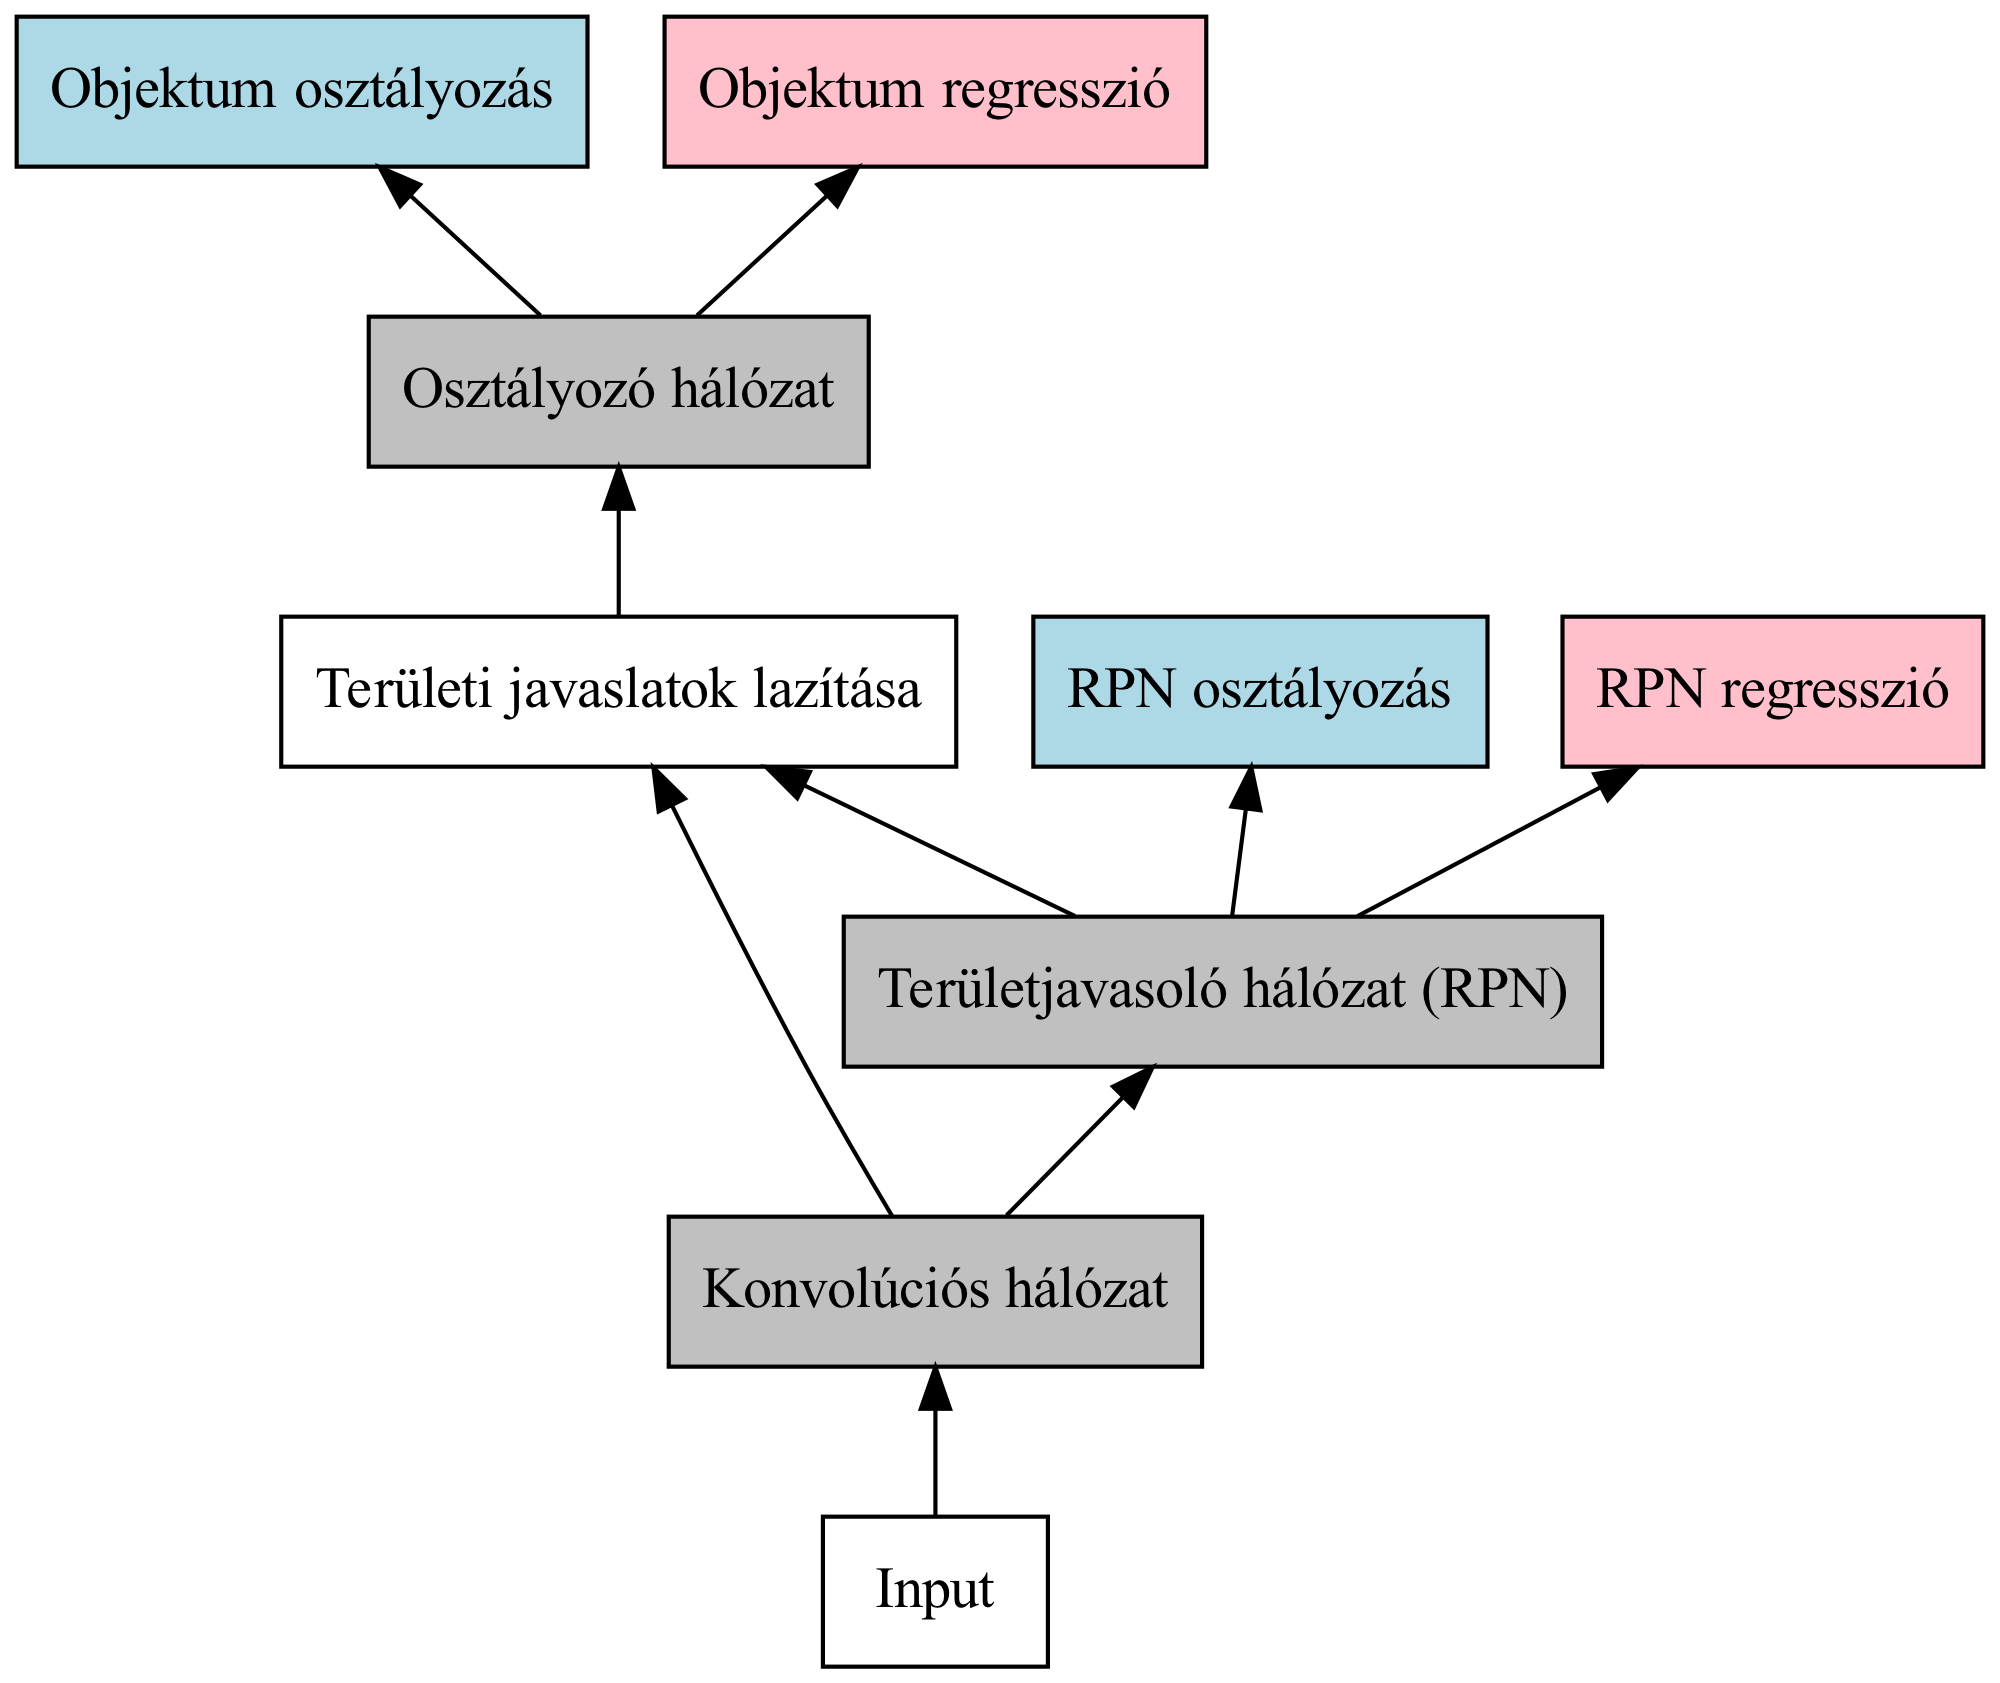
\includegraphics[height=7cm, width=7cm, keepaspectratio]{../../8_od/doc/graphs/od_7.png}}
\only<2>{Egyed szegmentáló hálózat (Mask R-CNN)\par\smallskip
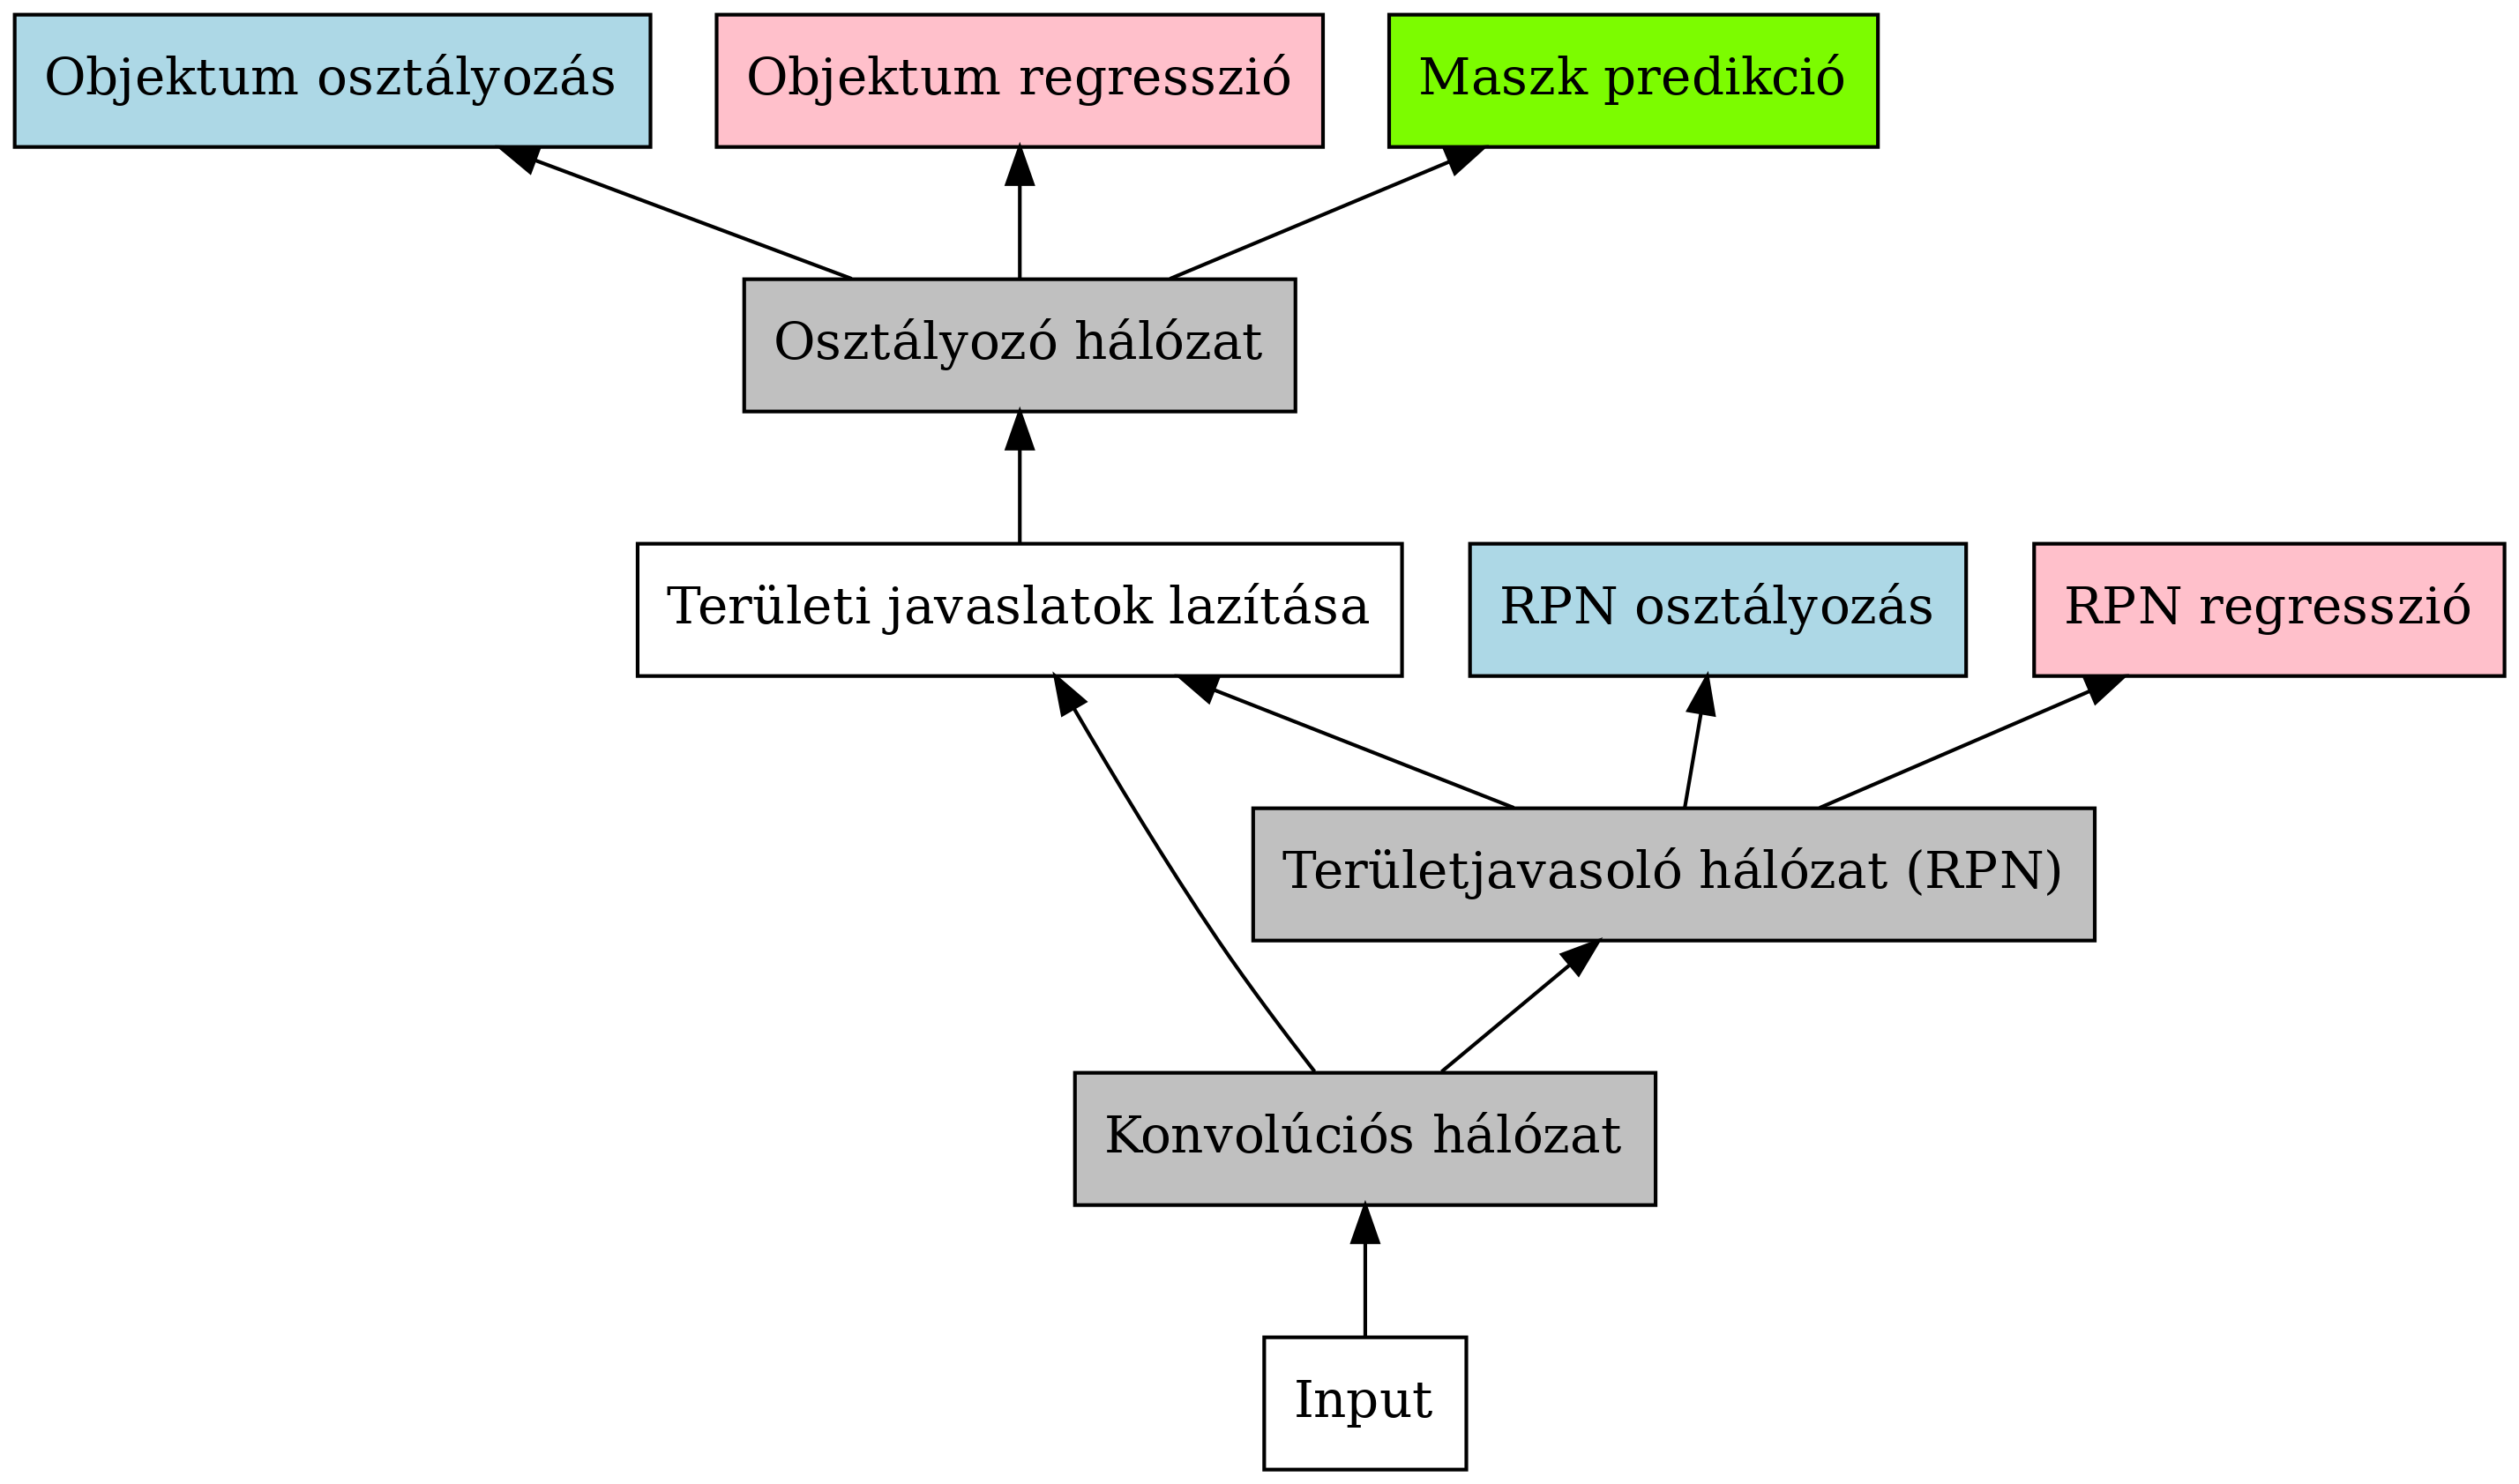
\includegraphics[height=7cm, width=7cm, keepaspectratio]{graphs/instance_2.png}}
\end{center}
\end{column}
\end{columns}
\end{frame}

\begin{frame}{Mask R-CNN architektúra}
\begin{columns}
\begin{column}{.4\textwidth}
A Mask R-CNN architektúra egy \textbf{továbbfejlesztése a Faster R-CNN keretrendszernek}, ami az egyed szegmentálásra specializálódott.\par\smallskip
A hálózat egy \textbf{maszk fejjel} (output hálózattal) képes osztályozni az egyes pixeleket. A hálózatnak ezen feje a területi javaslatok igazítása után képes \textbf{pixelszintű maszkokat megbecsülni minden objektumra}.
\end{column}
\begin{column}{.6\textwidth}
\begin{center}
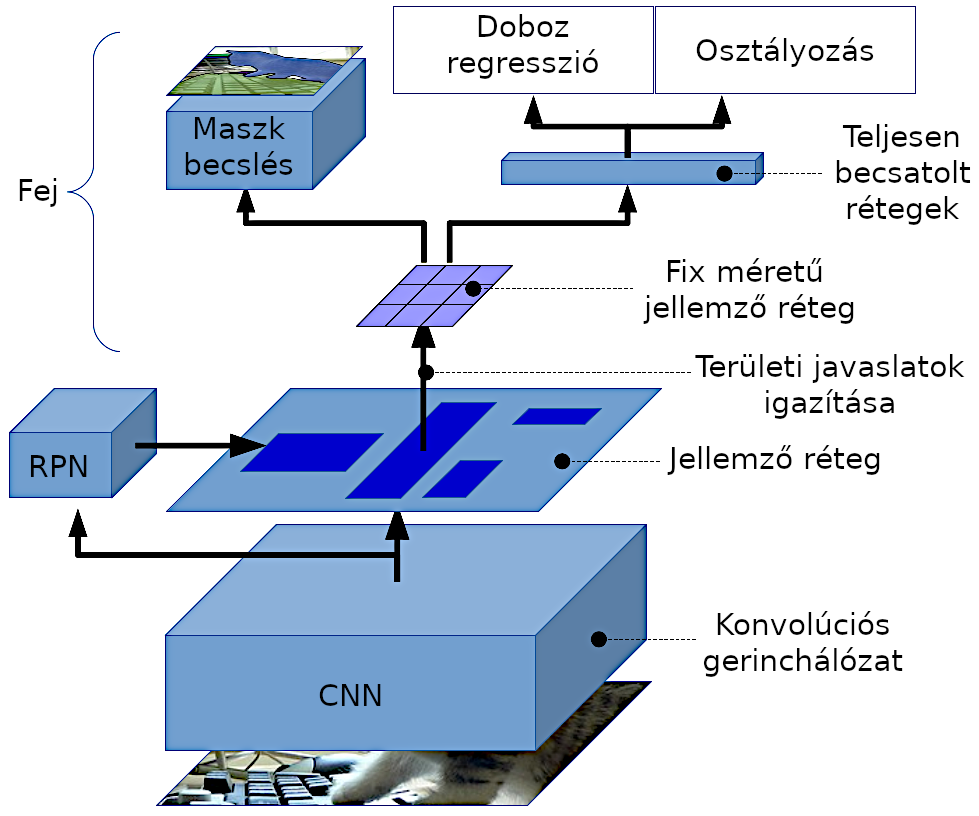
\includegraphics[height=8cm, width=8cm, keepaspectratio]{images/instance_17.png}
\end{center}
\end{column}
\end{columns}
\end{frame}

\begin{frame}{Területi javaslatok lazítása}
A területi javaslat lazítás (RoI pooling) felosztja az inputként érkező javasolt területet egy $n \cdot n$ méretű cellára, amelyeket \textbf{egy előre definiált háló határoz meg}. A felosztott régiókon \textbf{max. pooling segítségével dimenziót csökkent} majd átadja az eredményt a következő rétegnek.
\begin{center}
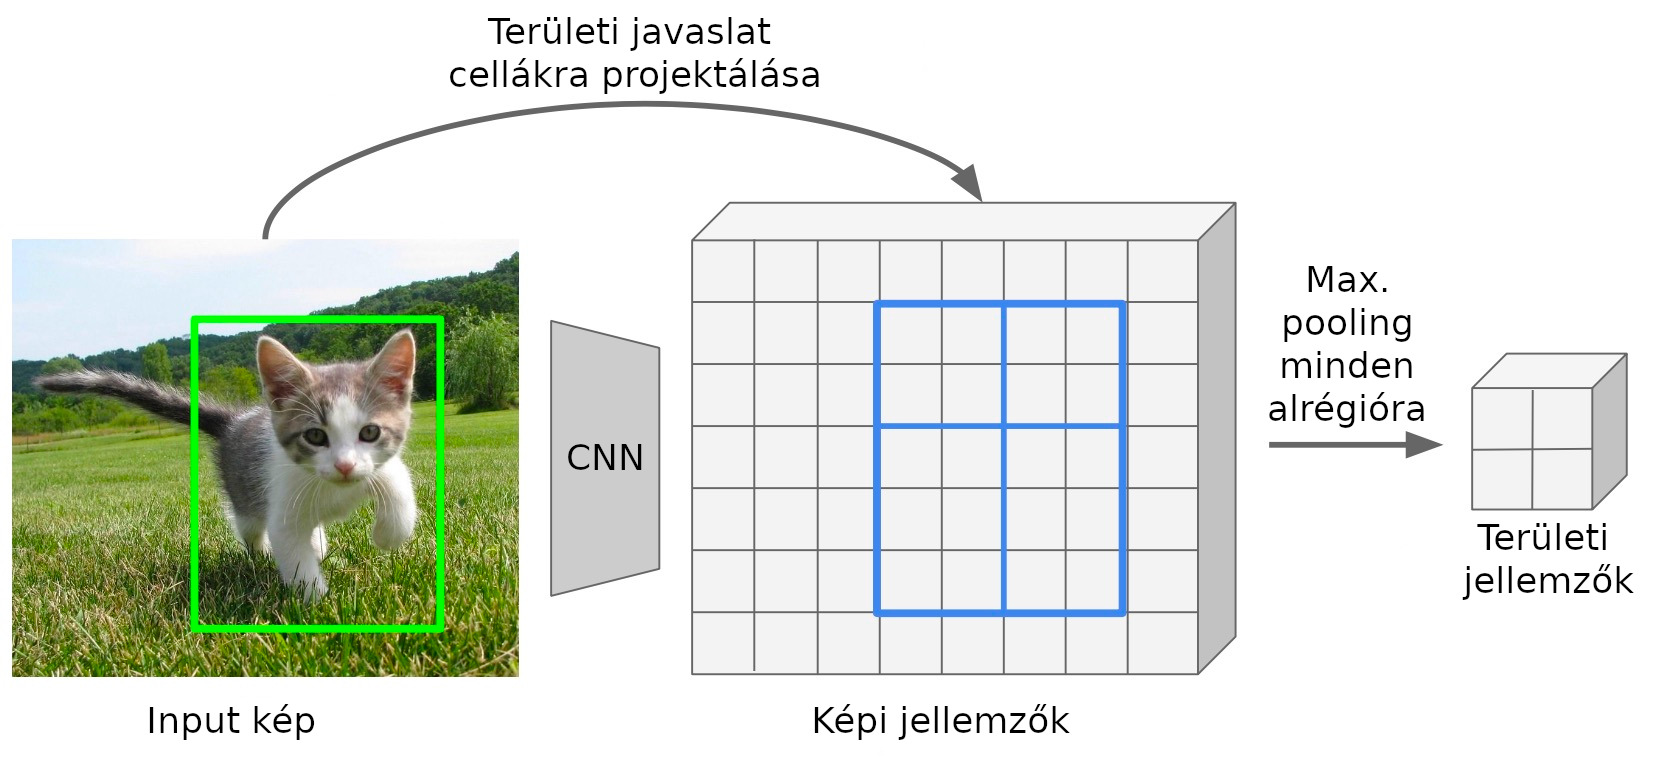
\includegraphics[height=7cm, width=11cm, keepaspectratio]{images/instance_18.png}
\end{center}
\end{frame}

\begin{frame}{Területi javaslatok igazítása}
A területi javaslat igazítás (RoI align) a lazítás továbbfejlesztésének tekinthető. Az igazító eljárás \textbf{nincs előre meghatározott cellahálóhoz kötve}, ezért a becsült értékek pontosabban illeszkednek az objektumokra. A mintavételezés itt \textbf{egyenletes intervallumokban történik, bilineáris interpoláció} segítségével.
\begin{center}
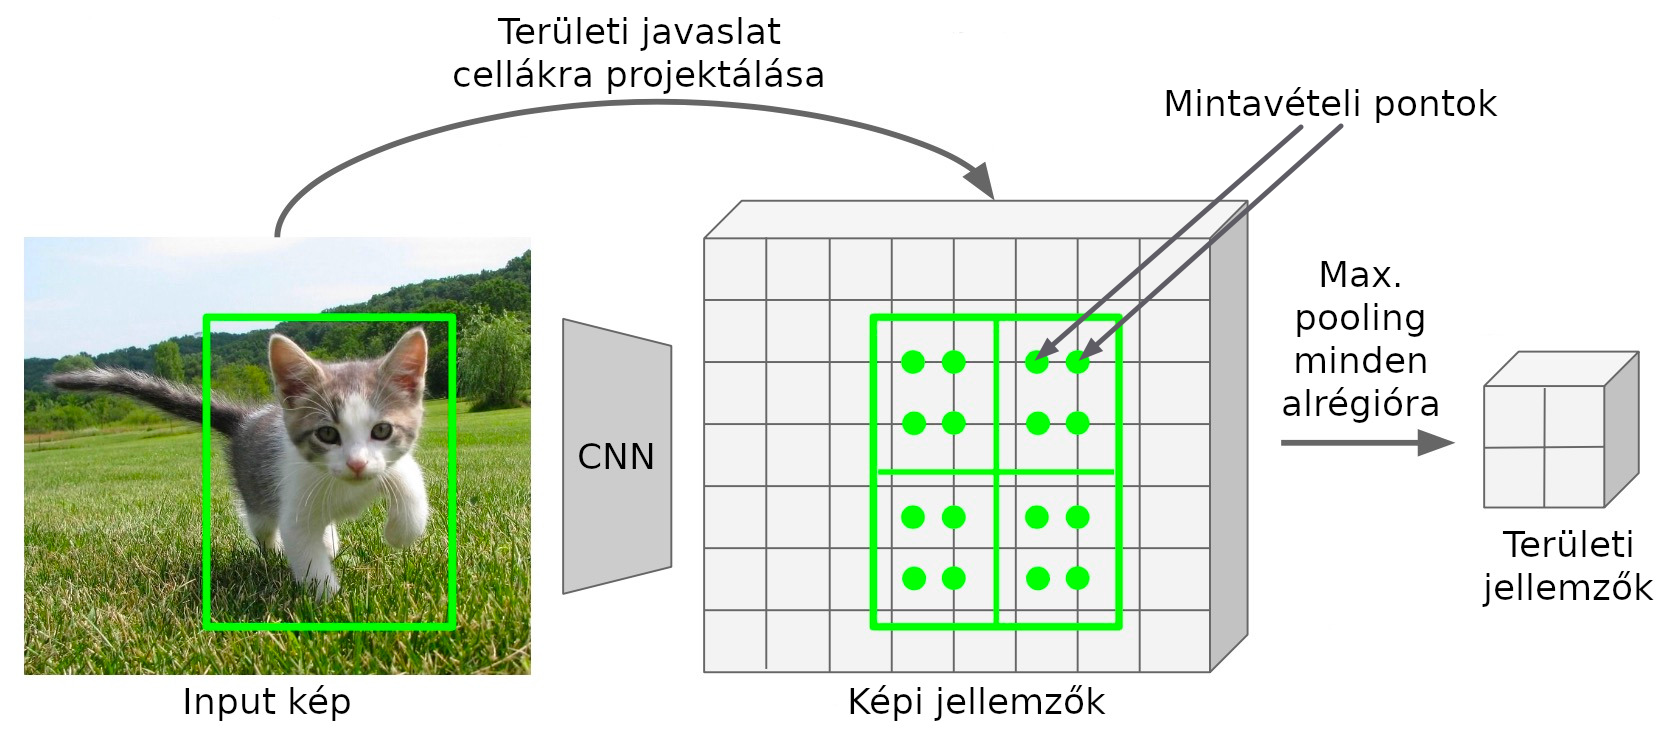
\includegraphics[height=7cm, width=11cm, keepaspectratio]{images/instance_19.png}
\end{center}
\end{frame}

\begin{frame}{Nem-maximális elnyomás (NMS)}
Az NMS feladata utólag feldolgozni a kereteződobozokra adott predikciókat úgy, hogy eltávolítsa a redundáns vagy átfedésben álló dobozokat. Az NMS folyamata:
\begin{columns}
\begin{column}{.6\textwidth}
\begin{enumerate}
	\item \textbf{Rendezés}: Dobozok rendezése a becslések valószínűsége szerint.
	\item \textbf{Iteráció}: A legbiztosabb doboz és az összes többi doboz közötti IoU kiszámolása.
	\item \textbf{Küszöbölés}: Azok a dobozok, amelyek adott küszöb feletti valószínűségekkel rendelkeznek, redundánsnak számítanak. 
	\item \textbf{Eldobás}: A redundáns kereteződobozok eldobása.
	\item \textbf{Ismétlés}: A folyamat megismétlődik az összes többi kereteződobozra. 
\end{enumerate}
\end{column}
\begin{column}{.4\textwidth}
\begin{center}
\includegraphics<1>[height=7cm, width=6cm, keepaspectratio]{images/instance_20.png}
\includegraphics<2>[height=7cm, width=6cm, keepaspectratio]{images/instance_21.png}
\end{center}
\end{column}
\end{columns}
\end{frame}

\section{Pózfelismerés}

\begin{frame}
\tableofcontents[currentsection]
\end{frame}

\begin{frame}{Emberi pózfelismerés alapjai}
A pózfelismerés célja az emberi végtagok lokalizálása képeken és videókon. A modell felismeri az emberi test fontosabb pontjait (\textbf{kulcspontjait}) és ezeket köti össze a póz rekonstruálása érdekében. Fontosabb \textbf{kulcspontok} a fej, fülek, nyak, vállak, csípők stb...
\begin{center}
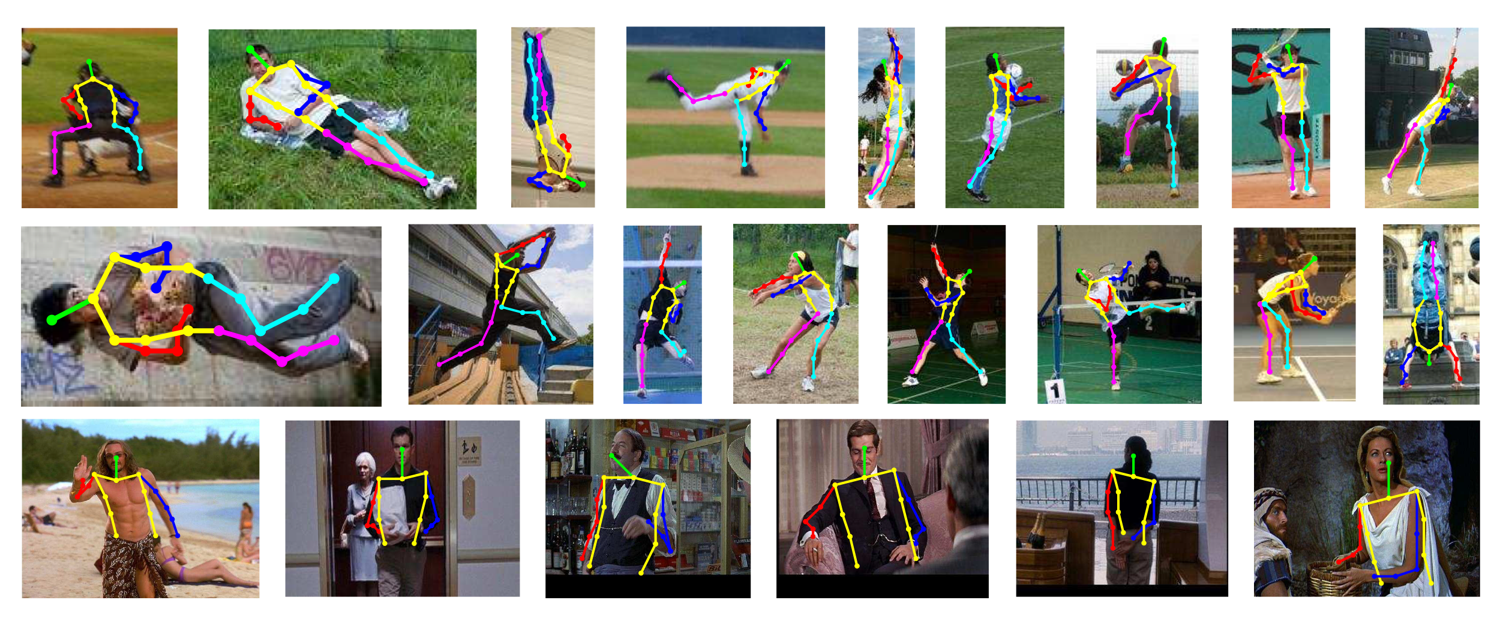
\includegraphics[height=7cm, width=12cm, keepaspectratio]{images/instance_22.png}
\end{center}
\end{frame}

\begin{frame}{Kulcspontok}
A leginkább elterjedt egységes jelölés 18 különböző kulcspontot különböztet meg (ez nem minden modellnél azonos): 
\begin{columns}
\begin{column}{.5\textwidth}
\begin{column}{.5\textwidth}
\begin{enumerate}
	\setcounter{enumi}{-1}
	\item Orr
	\item Nyak
	\item Jobb váll
	\item Jobb könyök
	\item Jobb csukló
	\item Bal váll
	\item Bal könyök
	\item Bal csukló
	\item Jobb csípő
\end{enumerate}
\end{column}
\begin{column}{.5\textwidth}
\begin{enumerate}
	\setcounter{enumi}{8}
	\item Jobb térd
	\item Jobb boka
	\item Bal csípő
	\item Bal térd
	\item Bal boka
	\item Jobb szem
	\item Bal szem
	\item Jobb fül
	\item Bal fül
\end{enumerate}
\end{column}
\end{column}
\begin{column}{.5\textwidth}
\begin{center}
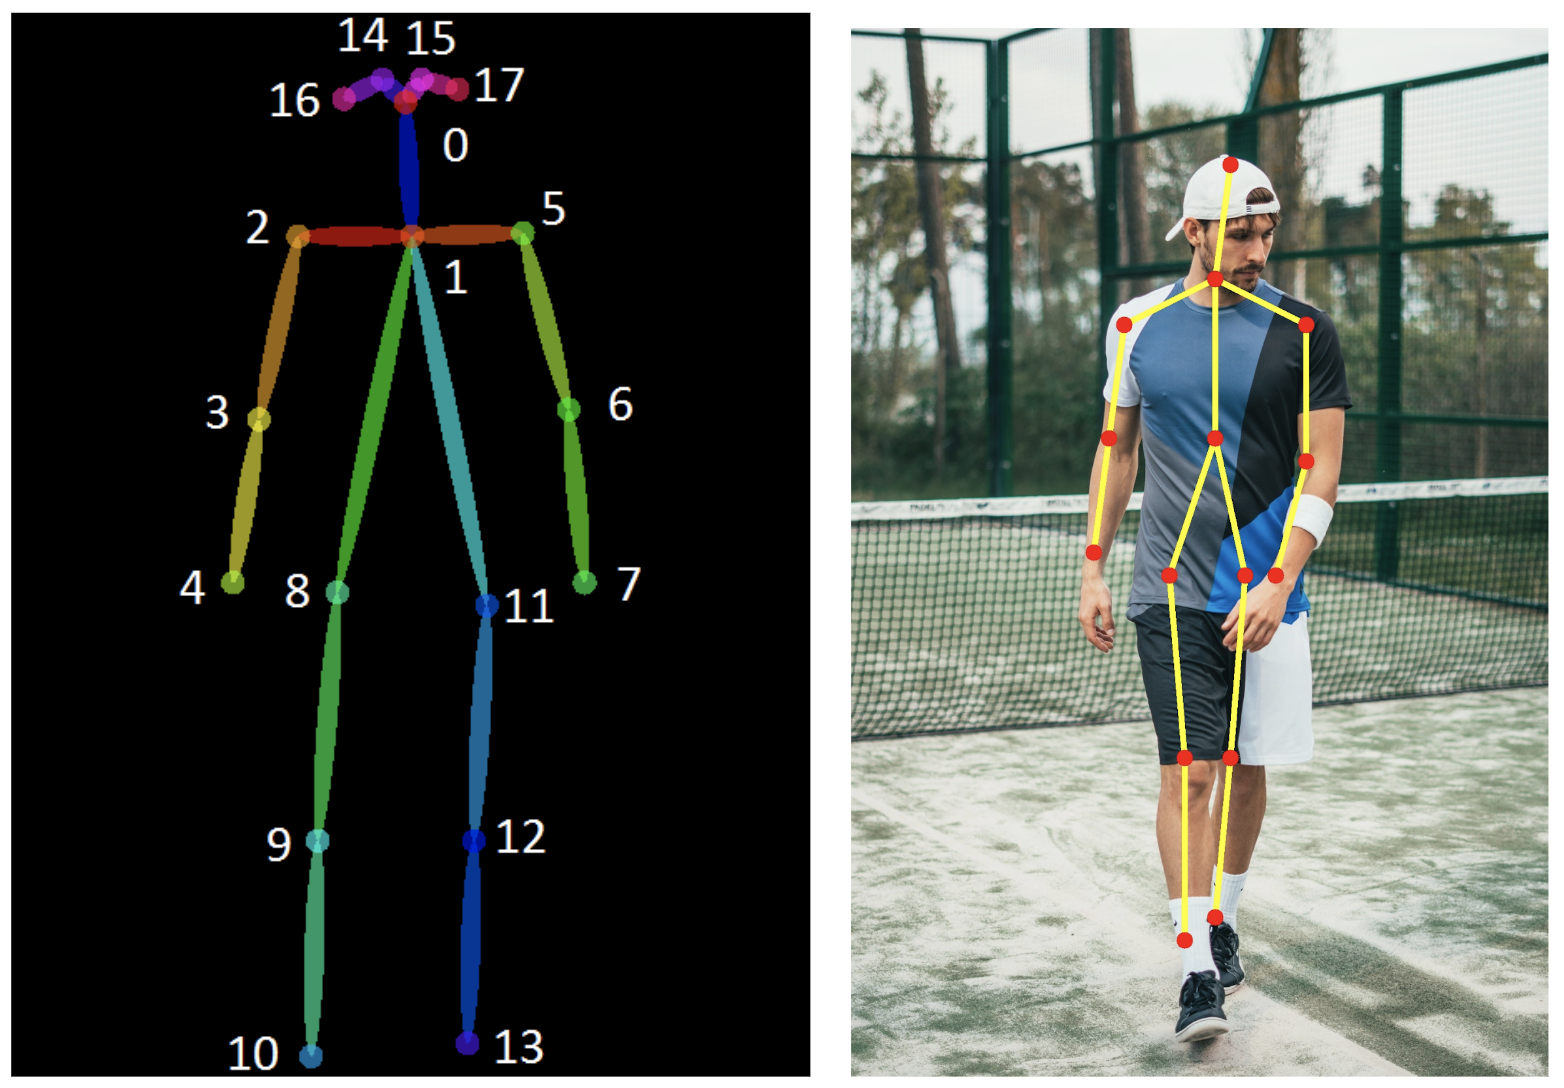
\includegraphics[height=7cm, width=7cm, keepaspectratio]{images/instance_23.png}
\end{center}
\end{column}
\end{columns}
\end{frame}

\begin{frame}{Testmodellek fajtái}
\begin{columns}
\begin{column}{.5\textwidth}
\begin{itemize}
	\item \textbf{Kinetikus}: Legjobb alkalmazása dinamikus, mozgással és testtartással kapcsolatos információ bányászására szolgál. 
	\item \textbf{Síkbeli}: Egy egyszerűsített reprezentáció amely abban az esetben hasznos, amikor valamilyen mozgás a síkban történik. 
	\item \textbf{Volumetrikus}: Egy összetett, 3D reprezentációja az emberi testnek, ami a test geometrikus elrendezését és térbeli eloszlását hivatott a lehető legpontosabban rekonstruálni. 
\end{itemize}
\end{column}
\begin{column}{.5\textwidth}
\begin{center}
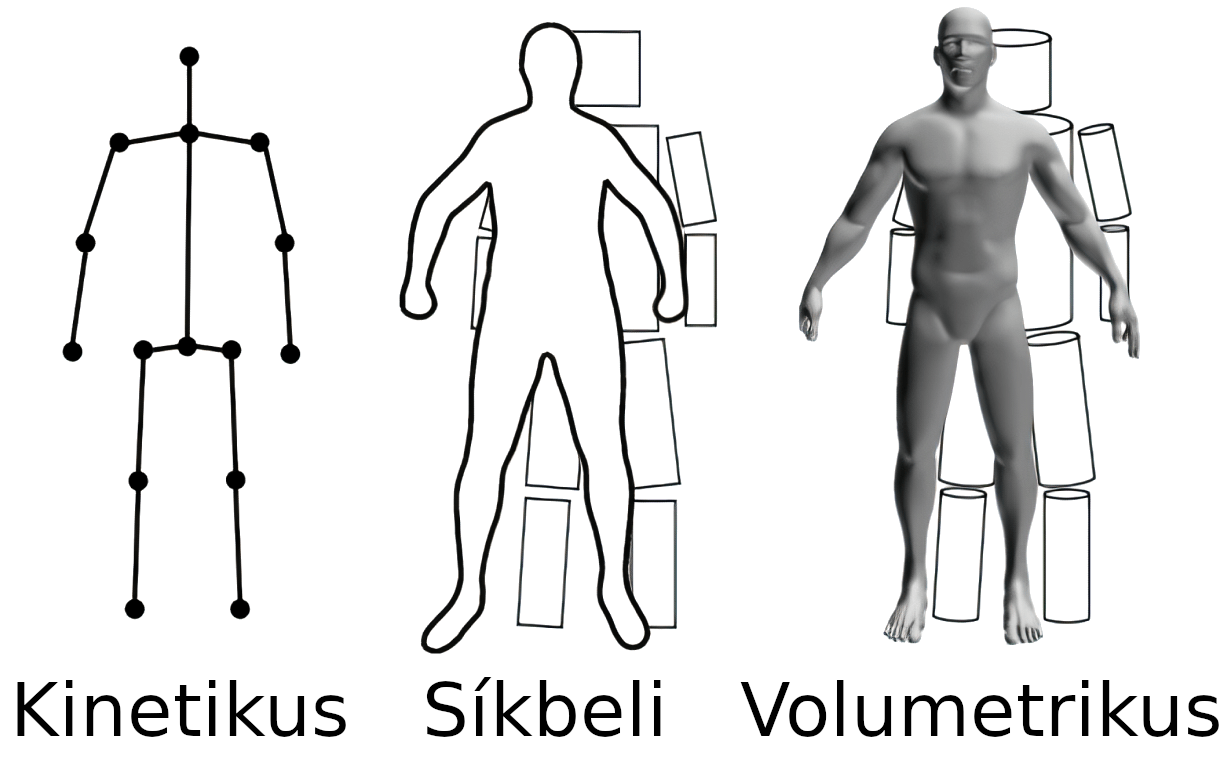
\includegraphics[height=8cm, width=7cm, keepaspectratio]{images/instance_25.png}
\end{center}
\end{column}
\end{columns}
\end{frame}

\begin{frame}{Klasszikus hozzáállások a pózbecsléshez}
Az eredeti, \textbf{Pictorial Structures} keretrendszeren alapuló hozzáállás az emberi testet \textbf{különálló, merev részekként} fogta fel, amely egy \textbf{deformálható, laza konfigurációban helyezkednek el a képen}. Minden rész egy sablonként jelenik meg, amelyet az algoritmus megpróbál valamely képrészhez hozzátársítani.\par\medskip
\begin{columns}
\begin{column}{.5\textwidth}
Az ebből adódó struktúra nagyon \textbf{jól tudja modellezni a különböző részek egymáshoz illeszkedését} ami fontos az emberi pózbecslésben, viszont \textbf{nagyon függ a képi jellemzőktől}. Ha valamely testrész nem tökéletesen felismerhető, az illesztés összeomlik. 
\end{column}
\begin{column}{.5\textwidth}
\begin{center}
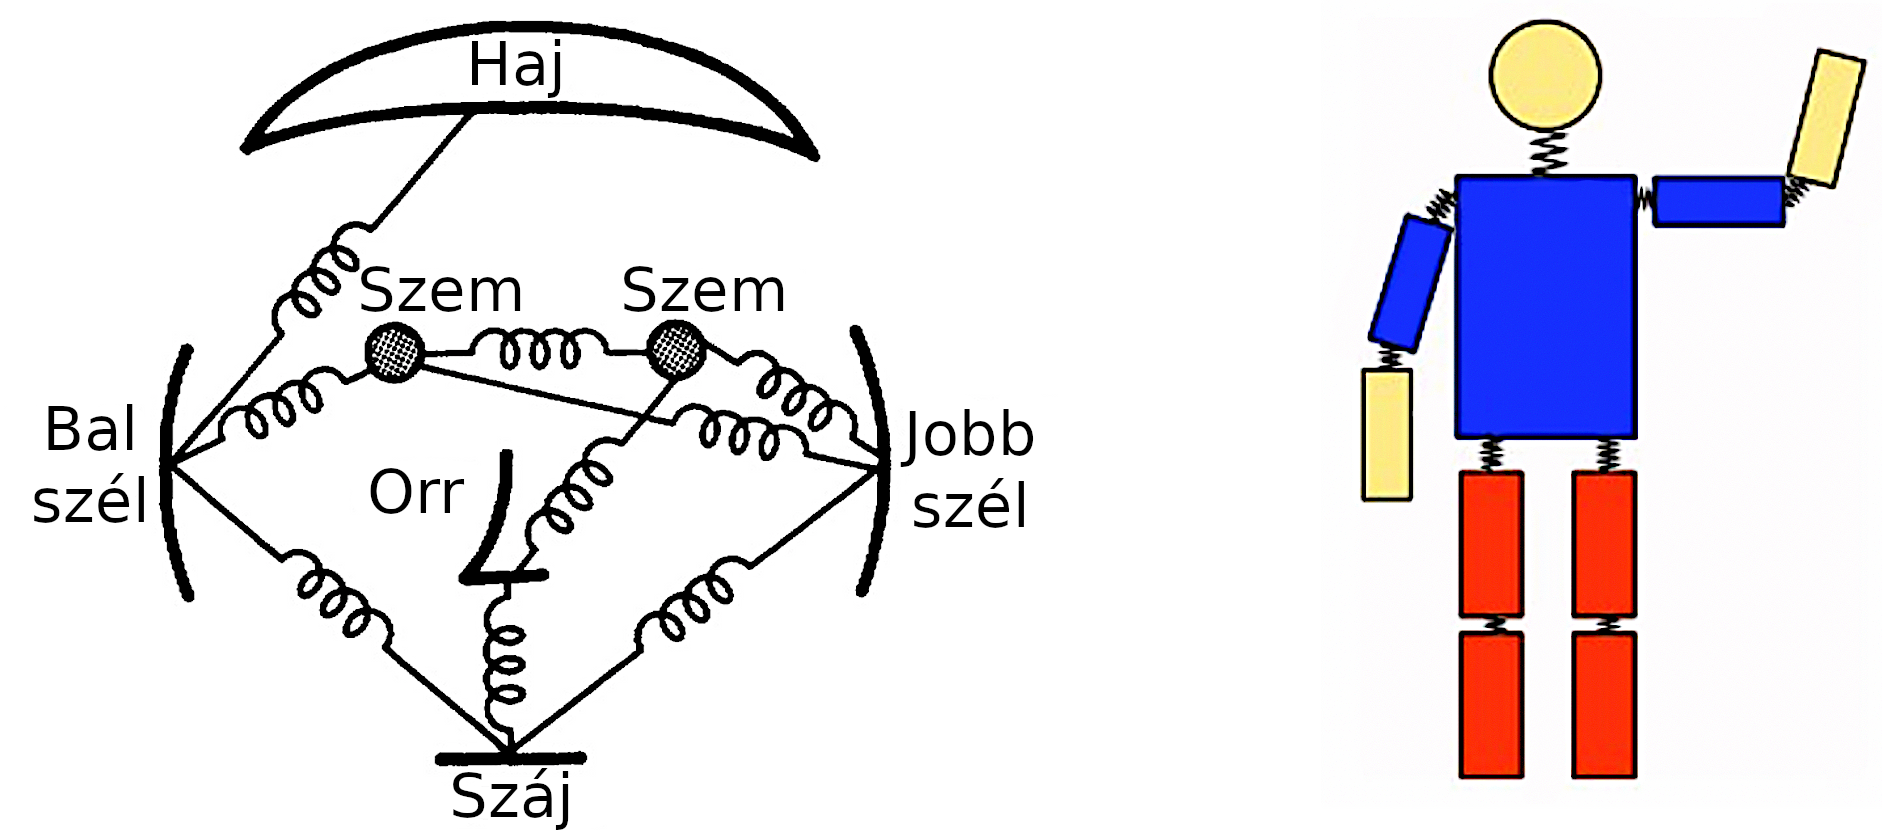
\includegraphics[height=7cm, width=7cm, keepaspectratio]{images/instance_24.png}
\end{center}
\end{column}
\end{columns}
\end{frame}

\begin{frame}{Modern megközelítés: OpenPose architektúra}
Az OpenPose egyike a legkorszerűbb valós idejű pózfelismerő modelleknek az egyike. Első lépésben minden testrészhez egy \textbf{magabiztossági térképet} becsül meg ami megadja, a kép mely részén a legvalószínűbb a jelenléte. Ezután a becsült testrészeket \textbf{irányított kapcsolási mezőkkel} párosítja őket kettesével.
\begin{center}
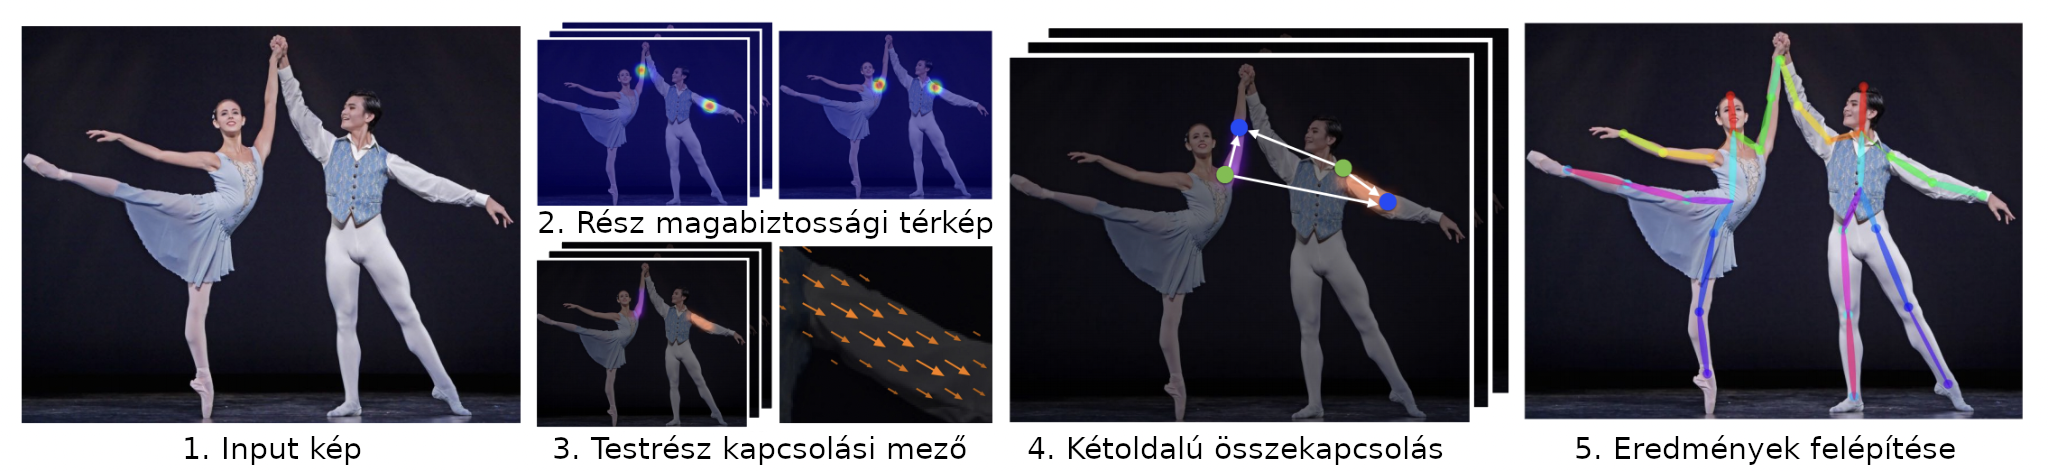
\includegraphics[height=7cm, width=14cm, keepaspectratio]{images/instance_26.png}
\end{center}
\end{frame}

\begin{frame}{OpenPose részletei}
\begin{columns}
\begin{column}{.35\textwidth}
Az OpenPose \textbf{minden testrész magabiztossági mezőt egyenként} becsül meg a testrészekre, majd a \textbf{kapcsolási mezők segítségével meghatározza ezeknek egymáshoz való viszonyát}. A kapcsolási mezőket és a magabiztossági jellemzőket egymástól függetlenül is lehetséges megbecsülni.
\end{column}
\begin{column}{.65\textwidth}
\begin{center}
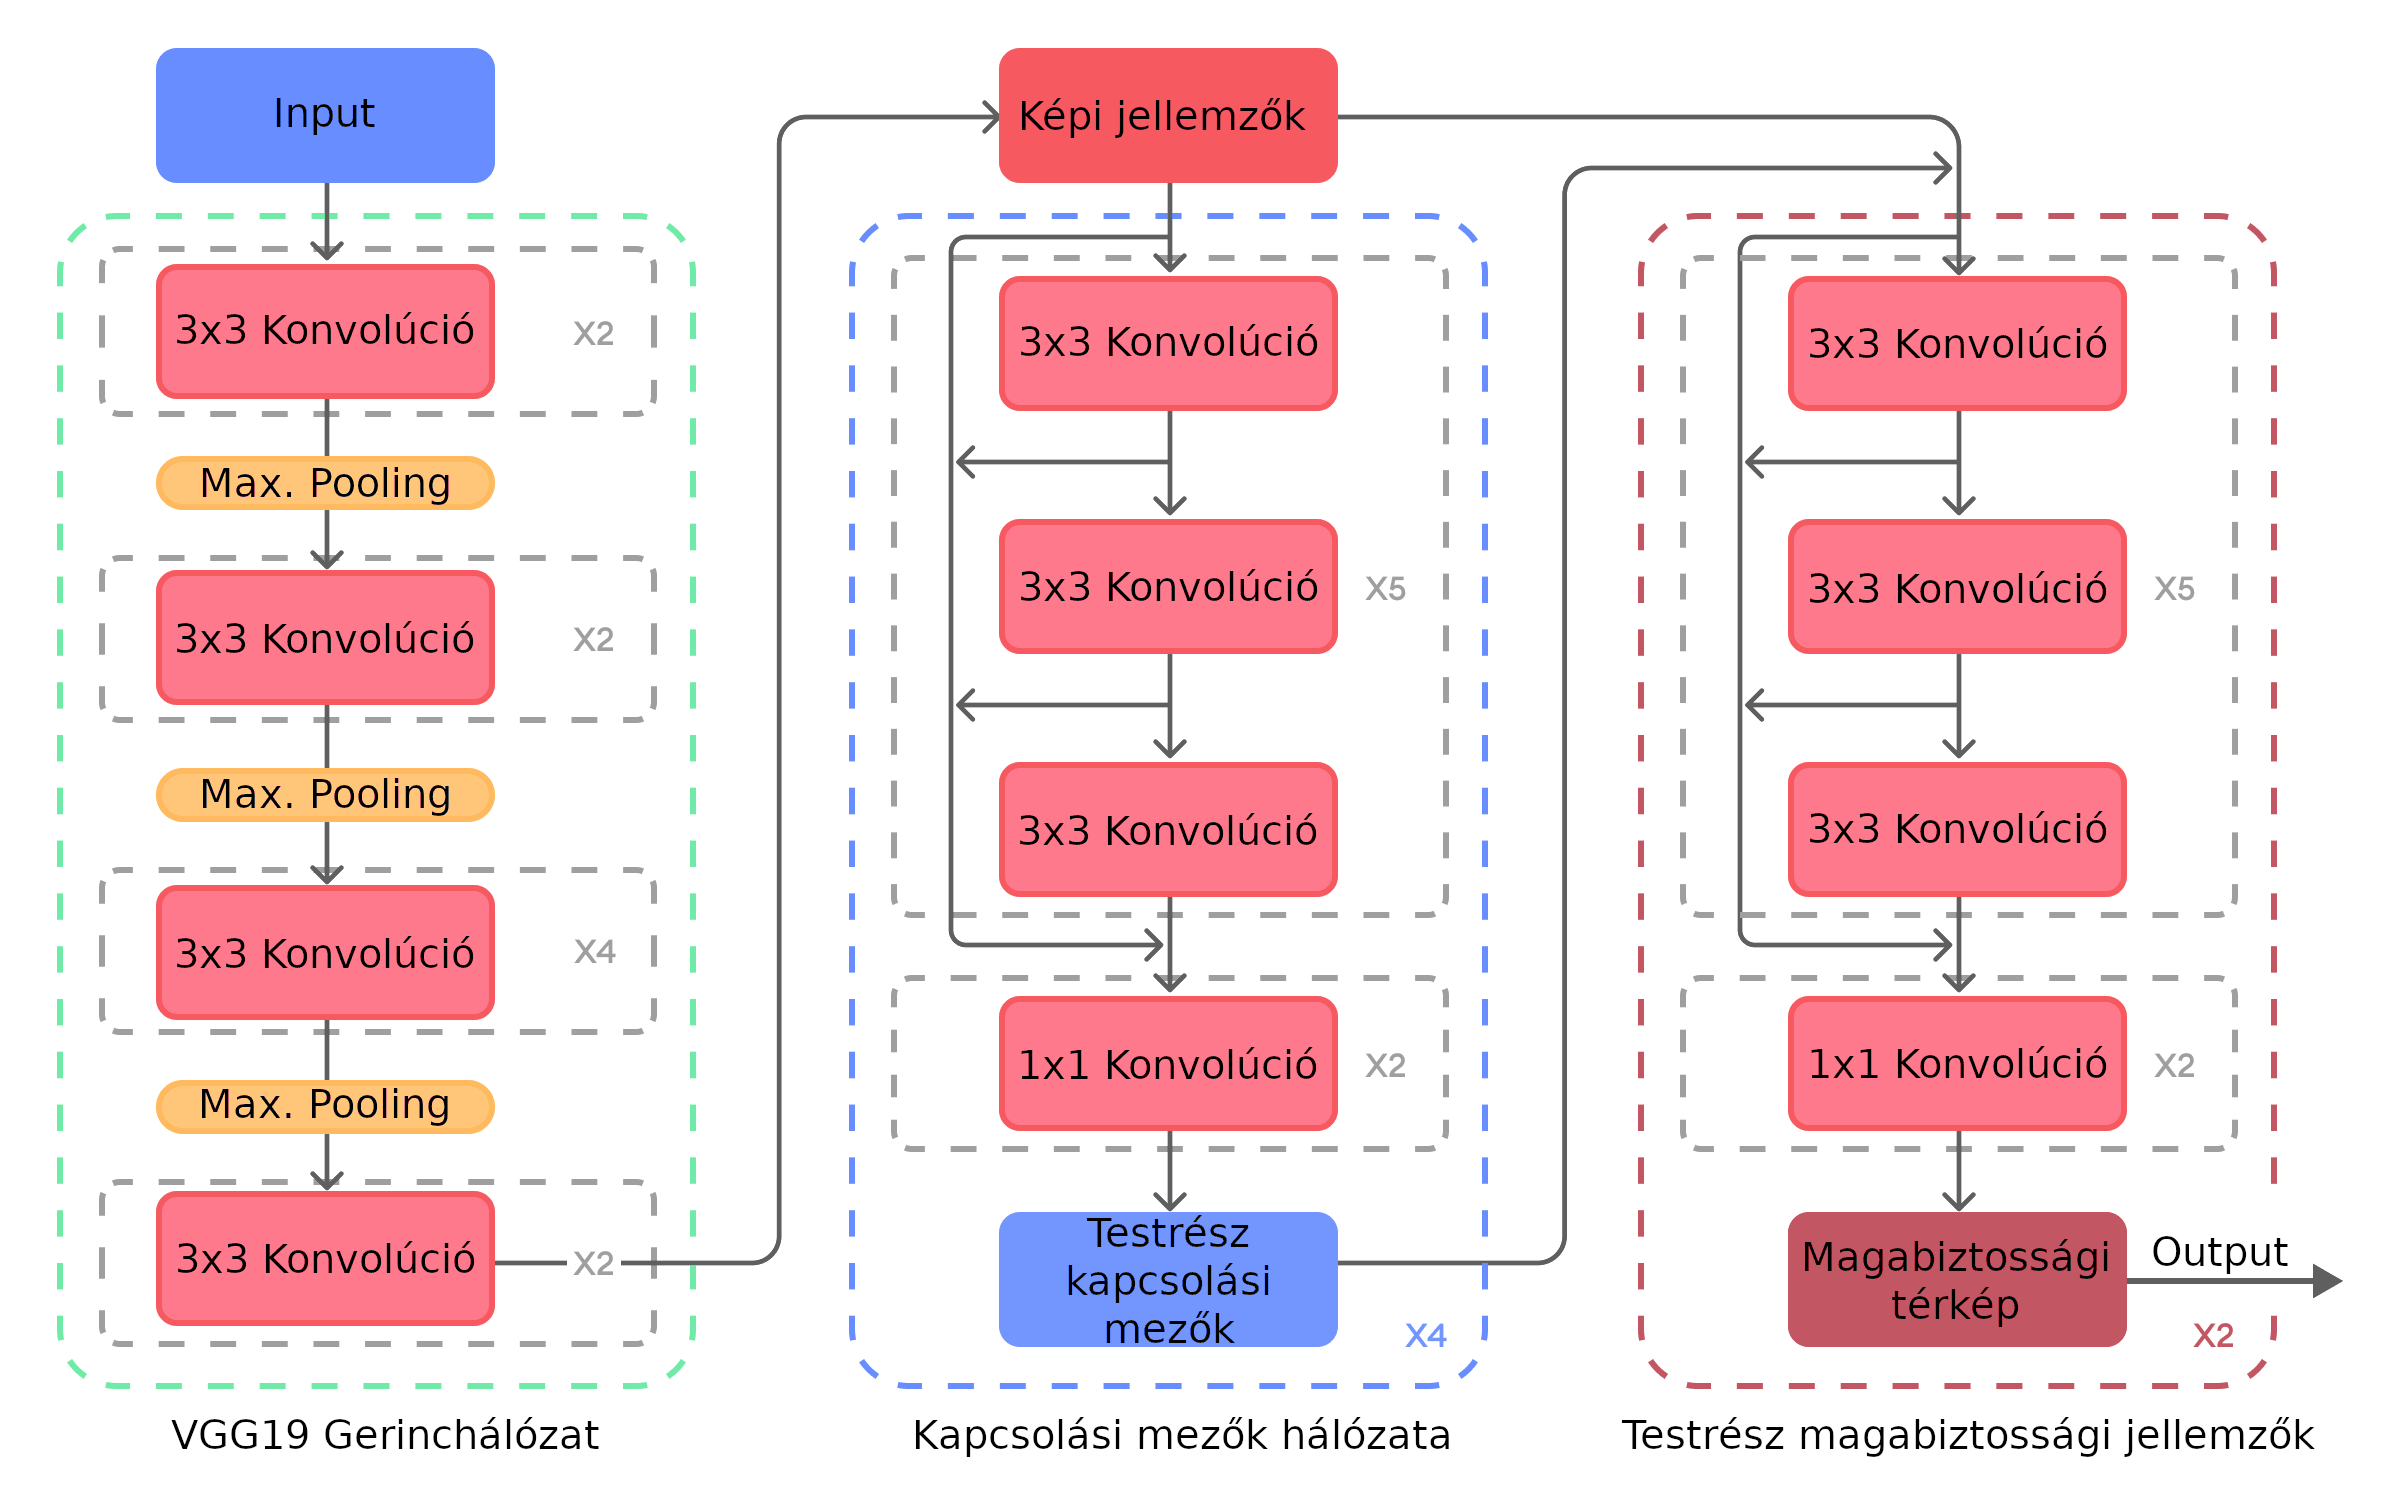
\includegraphics[height=7cm, width=9.5cm, keepaspectratio]{images/instance_27.png}
\end{center}
\end{column}
\end{columns}
\end{frame}

\end{document}


















